% feynlab v1.0 -- presentation slides (LaTeX Beamer)
% Build:  latexmk -pdf feynlab_slides.tex      (needs the PNGs in ../../benchmarks/figures, ../figures and ./figures)
\documentclass[aspectratio=169,10pt]{beamer}
\usepackage[utf8]{inputenc}
\usepackage[T1]{fontenc}
\usepackage{lmodern}
\usepackage{amsmath,amssymb,bm}
\usepackage{booktabs,array,multirow}
\usepackage{graphicx}
\usepackage{tikz}
\usetikzlibrary{arrows.meta,decorations.pathmorphing,decorations.markings,positioning,calc,shapes.geometric,fit,backgrounds}
\graphicspath{{figures/}{../../benchmarks/figures/}{../../benchmarks/ed_dmft/}{../figures/}}

% ------------------------------------------------------------------ palette
\definecolor{ink}{HTML}{1F1F1E}
\definecolor{muted}{HTML}{6B6A64}
\definecolor{paper}{HTML}{FAF9F6}
\definecolor{rule}{HTML}{E6E5E0}
\definecolor{brand}{HTML}{1D3557}
\definecolor{accent}{HTML}{2A78D6}
% physical-quantity colours (used consistently in every equation)
\definecolor{cG}{HTML}{1F6FD1}    % Green's functions, propagators
\definecolor{cS}{HTML}{E0601F}    % self-energies
\definecolor{cU}{HTML}{C0262D}    % interactions, impurity potentials, T-matrix
\definecolor{cH}{HTML}{138A5E}    % Hamiltonians and one-body operators (H, epsilon_k, S, L, O)
\definecolor{cB}{HTML}{7B4FBF}    % geometry: Berry curvature, orbital moment, dipole
\definecolor{cV}{HTML}{B07800}    % velocities and currents
\definecolor{cT}{HTML}{0E8C99}    % temperature, frequencies, imaginary time
\definecolor{cD}{HTML}{8A5A2B}    % hybridization / bath
\definecolor{cX}{HTML}{A61E6B}    % response functions, conductivities, susceptibilities

\newcommand{\G}[1][]{{\color{cG}G_{#1}}}
\newcommand{\Gz}[1][]{{\color{cG}G^{0}_{#1}}}
\newcommand{\Gw}{{\color{cG}\mathcal{G}_0}}
\newcommand{\Sig}[1][]{{\color{cS}\Sigma_{#1}}}
\newcommand{\U}{{\color{cU}U}}
\newcommand{\J}{{\color{cU}J}}
\newcommand{\Vimp}{{\color{cU}V_0}}
\newcommand{\Tm}{{\color{cU}T}}
\newcommand{\Ham}{{\color{cH}H}}
\newcommand{\ek}{{\color{cH}\varepsilon_{\mathbf k}}}
\newcommand{\Op}{{\color{cH}\hat O}}
\newcommand{\Om}{{\color{cB}\Omega}}
\newcommand{\morb}{{\color{cB}m}}
\newcommand{\Dip}{{\color{cB}D}}
\newcommand{\vel}[1]{{\color{cV}v^{#1}}}
\newcommand{\jcur}[1]{{\color{cV}J^{#1}}}
\newcommand{\iw}{{\color{cT}i\omega_n}}
\newcommand{\tauv}{{\color{cT}\tau}}
\newcommand{\bet}{{\color{cT}\beta}}
\newcommand{\Hyb}{{\color{cD}\Delta}}
\newcommand{\chiq}{{\color{cX}\chi}}
\newcommand{\sxy}{{\color{cX}\sigma_{xy}}}

% ------------------------------------------------------------------ theme
\setbeamercolor{background canvas}{bg=white}
\setbeamercolor{normal text}{fg=ink}
\setbeamercolor{frametitle}{fg=brand,bg=white}
\setbeamercolor{title}{fg=white}
\setbeamercolor{subtitle}{fg=white!85!brand}
\setbeamercolor{structure}{fg=accent}
\setbeamercolor{block title}{fg=white,bg=brand}
\setbeamercolor{block body}{bg=paper}
\setbeamercolor{block title alerted}{fg=white,bg=cU}
\setbeamercolor{block body alerted}{bg=cU!6}
\setbeamercolor{block title example}{fg=white,bg=cH}
\setbeamercolor{block body example}{bg=cH!6}
\setbeamerfont{frametitle}{size=\Large,series=\bfseries}
\setbeamertemplate{navigation symbols}{}
\setbeamertemplate{itemize item}{\color{accent}$\blacktriangleright$}
\setbeamertemplate{itemize subitem}{\color{muted}--}
\setbeamertemplate{blocks}[rounded][shadow=false]
\setbeamertemplate{frametitle}{%
  \vspace*{0.35cm}\hspace*{-0.05cm}\usebeamerfont{frametitle}\usebeamercolor[fg]{frametitle}\insertframetitle
  \ifx\insertframesubtitle\@empty\else\\[-1pt]{\normalsize\color{muted}\insertframesubtitle}\fi
  \par\vspace*{-0.1cm}{\color{accent}\rule{1.6cm}{2pt}}}
\setbeamertemplate{footline}{%
  \leavevmode\hbox to\paperwidth{\hspace{0.4cm}{\color{muted}\tiny feynlab v1.2 \,|\, \insertsectionhead}\hfill{\color{muted}\tiny\insertframenumber/\inserttotalframenumber}\hspace{0.4cm}}\vspace{0.18cm}}
\AtBeginSection[]{%
  \begin{frame}[plain]
  \begin{tikzpicture}[remember picture,overlay]
   \fill[brand] (current page.south west) rectangle (current page.north east);
   \node[anchor=south west,text=white,font=\huge\bfseries,text width=13cm,align=left] at ($(current page.west)+(1.2,0.0)$) {\insertsectionhead};
   \fill[accent] ($(current page.west)+(1.25,-0.25)$) rectangle ++(1.6,0.07);
   \node[anchor=north west,text=white!70!brand,font=\small] at ($(current page.west)+(1.2,-0.45)$) {Section \thesection};
  \end{tikzpicture}
  \end{frame}}

\tikzset{
  fermion/.style={thick,cG,postaction={decorate},decoration={markings,mark=at position .55 with {\arrow{Stealth[length=5pt]}}}},
  dfermion/.style={double,double distance=1.3pt,thick,cG,postaction={decorate},decoration={markings,mark=at position .55 with {\arrow[cG]{Stealth[length=6pt]}}}},
  inter/.style={thick,cU,decorate,decoration={snake,amplitude=1.6pt,segment length=5pt}},
  imp/.style={thick,cU,dashed},
  vtx/.style={circle,fill=ink,inner sep=1.1pt},
  sig/.style={circle,draw=cS,fill=cS!20,thick,minimum size=16pt,inner sep=0pt,font=\small\color{cS}},
  box/.style={rounded corners=3pt,draw=#1,fill=#1!8,thick,align=center,font=\footnotesize,inner sep=4pt},
}
\newcommand{\refcite}[1]{{\color{muted}\scriptsize[#1]}}
\newcommand{\ok}{{\color{cH}\checkmark}}

\title{\textbf{feynlab} v1.2}
\subtitle{Feynman diagrams, quantum Monte Carlo, many-body self-energies\\and anomalous/spin/orbital Hall transport in one validated Python package}
\author{Gokaran Shukla}
\institute{KAUST \quad\textbullet\quad github.com/Gokaran-Shukla/feynlab}
\date{November 2026}

\begin{document}

% ======================================================================== title
\begin{frame}[plain]
\begin{tikzpicture}[remember picture,overlay]
 \fill[brand] (current page.south west) rectangle (current page.north east);
 \fill[accent] ($(current page.south west)+(0,1.05)$) rectangle ($(current page.south east)+(0,1.12)$);
 \node[anchor=north west,text=white,font=\fontsize{40}{40}\selectfont\bfseries] at ($(current page.north west)+(1.0,-1.1)$) {feynlab \,\normalsize v1.2};
 \node[anchor=north west,text=white!85!brand,text width=11.5cm,font=\large] at ($(current page.north west)+(1.05,-2.6)$)
   {Feynman diagrams, quantum Monte Carlo, many-body self-energies and anomalous / spin / orbital Hall transport \textemdash{} in one validated Python package};
 \node[anchor=south west,text=white,font=\normalsize] at ($(current page.south west)+(1.05,1.6)$) {\textbf{Gokaran Shukla}\quad KAUST, Thuwal};
 \node[anchor=south west,text=white!70!brand,font=\scriptsize,align=left] at ($(current page.south west)+(1.05,0.2)$) {github.com/Gokaran-Shukla/feynlab\\[1pt] companion to R.\,D.\ Mattuck, \emph{A Guide to Feynman Diagrams in the Many-Body Problem}};
 % decorative self-energy diagram
 \begin{scope}[shift={($(current page.north east)+(-3.3,-4.6)$)},scale=1.25]
  \draw[thick,white!70!brand,postaction={decorate},decoration={markings,mark=at position .5 with {\arrow{Stealth}}}] (-1.6,0)--(-0.9,0);
  \draw[thick,white!70!brand,postaction={decorate},decoration={markings,mark=at position .5 with {\arrow{Stealth}}}] (-0.9,0)--(0.9,0);
  \draw[thick,white!70!brand,postaction={decorate},decoration={markings,mark=at position .5 with {\arrow{Stealth}}}] (0.9,0)--(1.6,0);
  \draw[thick,white!70!brand,postaction={decorate},decoration={markings,mark=at position .5 with {\arrow{Stealth}}}] (0.9,0) arc (0:180:0.9);
  \draw[thick,white!70!brand,postaction={decorate},decoration={markings,mark=at position .5 with {\arrow{Stealth}}}] (-0.9,0) arc (180:360:0.9);
  \draw[thick,accent!60!white,decorate,decoration={snake,amplitude=1.5pt,segment length=5pt}] (-0.9,0) -- (-0.9,0.0);
  \fill[white] (-0.9,0) circle (1.6pt) (0.9,0) circle (1.6pt);
 \end{scope}
\end{tikzpicture}
\end{frame}

\begin{frame}{Outline}
\begin{columns}[T]
\column{0.48\textwidth}
\begin{enumerate}\small
 \item Why feynlab \& architecture
 \item Colour code \& formalism (Matsubara, Dyson, FFT)
 \item Feynman diagrams: enumeration, evaluation, drawing
 \item Self-energy from weak to strong coupling
 \item Quantum Monte Carlo: CT-INT, CT-HYB
 \item Exact diagonalization \& the Mott transition
 \item Multi-orbital, DFT+DMFT, DCA, NRG
\end{enumerate}
\column{0.48\textwidth}
\begin{enumerate}\small\setcounter{enumi}{7}
 \item Analytic continuation
 \item Advanced diagrammatic Monte Carlo
 \item Hall transport: intrinsic, side jump, skew, crossed
 \item Orbitronics: OAM, BCD, Edelstein/SOT, 3D Wannier
 \item Robustness: errors, mixing, I/O, CLI, CI
 \item v1.1: closing every v1.0 limitation
 \item v1.2: charge self-consistency with Quantum ESPRESSO
 \item v1.3: $\lambda$-D$\Gamma$A and the remaining limits
 \item Benchmarks, limitations, learning material
\end{enumerate}
\end{columns}
\vfill
\begin{block}{In numbers}
\centering
\small
\begin{tabular}{ccc}
\textbf{35+} modules & \textbf{20} software tutorials & \textbf{22} book-chapter tutorials\\
\textbf{42} quizzes, \textbf{228} questions & \textbf{200+} benchmark rows & \textbf{60} unit tests
\end{tabular}
\end{block}
\end{frame}

% ======================================================================== 1
\section{Why feynlab}
\begin{frame}{Motivation}
\begin{columns}[T]
\column{0.55\textwidth}
\begin{itemize}
 \item Many-body codes are usually \emph{either} pedagogical \emph{or} research-grade: rarely both.
 \item Diagrammatic Monte Carlo, DMFT and Kubo transport live in separate ecosystems with incompatible conventions.
 \item Orbitronics needs \textbf{extrinsic} (side jump, skew, crossed) and \textbf{correlated} ingredients for \emph{orbital} currents --- not available in any public code.
 \item Results are trusted only if \textbf{every number} is compared with an exact or published value.
\end{itemize}
\column{0.42\textwidth}
\begin{block}{Design principles}
\begin{itemize}
 \item one convention for $\G$, $\Sig$, units
 \item every module $\leftrightarrow$ book chapter $\leftrightarrow$ tutorial $\leftrightarrow$ quiz
 \item every claim $\leftrightarrow$ a benchmark row with tolerance and citation
 \item limitations stated, not hidden
\end{itemize}
\end{block}
\end{columns}
\end{frame}

\begin{frame}{Architecture}
\centering
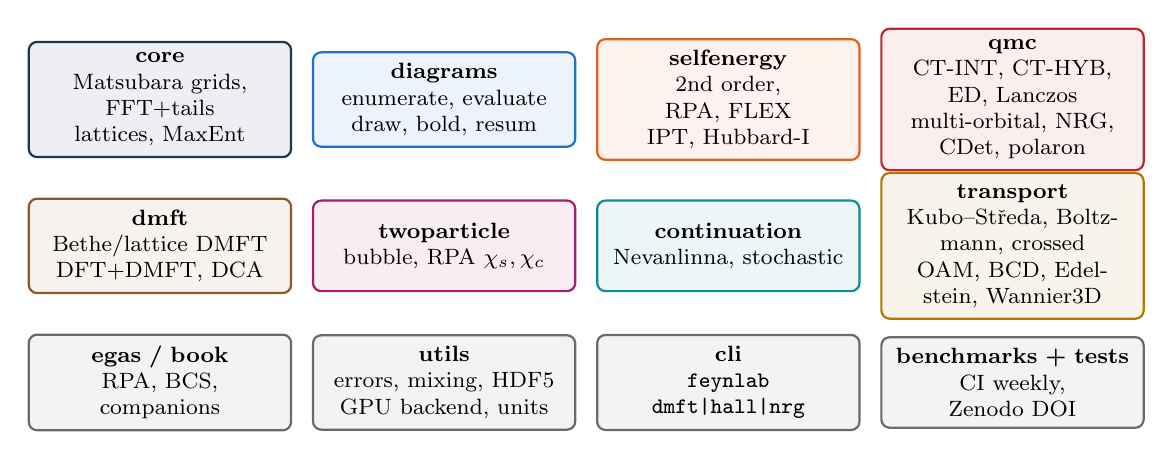
\begin{tikzpicture}[node distance=0.25cm and 0.25cm,every node/.append style={text width=3.05cm,font=\scriptsize}]
\node[box=brand,minimum height=1.15cm] (core) {\textbf{core}\\Matsubara grids, FFT+tails\\lattices, MaxEnt};
\node[box=cG,right=of core,minimum height=1.15cm] (diag) {\textbf{diagrams}\\enumerate, evaluate\\draw, bold, resum};
\node[box=cS,right=of diag,minimum height=1.15cm] (se) {\textbf{selfenergy}\\2nd order, RPA, FLEX\\IPT, Hubbard-I};
\node[box=cU,right=of se,minimum height=1.15cm] (qmc) {\textbf{qmc}\\CT-INT, CT-HYB, ED, Lanczos\\multi-orbital, NRG, CDet, polaron};
\node[box=cD,below=0.5cm of core,minimum height=1.15cm] (dmft) {\textbf{dmft}\\Bethe/lattice DMFT\\DFT+DMFT, DCA};
\node[box=cX,right=of dmft,minimum height=1.15cm] (two) {\textbf{twoparticle}\\bubble, RPA $\chi_s,\chi_c$};
\node[box=cT,right=of two,minimum height=1.15cm] (cont) {\textbf{continuation}\\Nevanlinna, stochastic};
\node[box=cV,right=of cont,minimum height=1.15cm] (tr) {\textbf{transport}\\Kubo--St\v{r}eda, Boltzmann, crossed\\OAM, BCD, Edelstein, Wannier3D};
\node[box=muted,below=0.5cm of dmft,minimum height=1.15cm] (eg) {\textbf{egas / book}\\RPA, BCS, companions};
\node[box=muted,right=of eg,minimum height=1.15cm] (ut) {\textbf{utils}\\errors, mixing, HDF5\\GPU backend, units};
\node[box=muted,right=of ut,minimum height=1.15cm] (cli) {\textbf{cli}\\\texttt{feynlab dmft|hall|nrg}};
\node[box=muted,right=of cli,minimum height=1.15cm] (bm) {\textbf{benchmarks + tests}\\CI weekly, Zenodo DOI};
\end{tikzpicture}
\vspace{0.3cm}

{\small Pure Python + NumPy/SciPy, Numba for Monte Carlo kernels, optional CuPy;\ \texttt{pip install -e .[gpu,docs]}}
\end{frame}

% ======================================================================== 2
\section{Colour code and formalism}
\begin{frame}{Colour code used in every equation}
\begin{columns}[T]
\column{0.5\textwidth}
\renewcommand{\arraystretch}{1.35}
\begin{tabular}{ll}
\toprule
colour & quantity \\ \midrule
\textcolor{cG}{\rule{8pt}{8pt}} blue & Green's functions $\G,\ \Gz,\ \Gw$ \\
\textcolor{cS}{\rule{8pt}{8pt}} orange & self-energies $\Sig$ \\
\textcolor{cU}{\rule{8pt}{8pt}} red & interactions $\U,\ \J,\ \Vimp,\ \Tm$ \\
\textcolor{cH}{\rule{8pt}{8pt}} green & Hamiltonians, operators $\Ham,\ \ek,\ \Op$ \\
\textcolor{cD}{\rule{8pt}{8pt}} brown & hybridization / bath $\Hyb$ \\
\bottomrule
\end{tabular}
\column{0.5\textwidth}
\renewcommand{\arraystretch}{1.35}
\begin{tabular}{ll}
\toprule
colour & quantity \\ \midrule
\textcolor{cT}{\rule{8pt}{8pt}} teal & $\bet,\ \iw,\ \tauv$ \\
\textcolor{cV}{\rule{8pt}{8pt}} gold & velocities, currents $\vel{x},\ \jcur{O}$ \\
\textcolor{cB}{\rule{8pt}{8pt}} purple & geometry $\Om,\ \morb,\ \Dip$ \\
\textcolor{cX}{\rule{8pt}{8pt}} magenta & responses $\chiq,\ \sxy$ \\
\bottomrule
\end{tabular}
\end{columns}
\vspace{0.4cm}
\begin{block}{Conventions (identical in all modules)}
$\G(\tauv)=-\langle T_\tau c(\tauv)c^\dagger(0)\rangle$, \quad
$\G(\iw)=\int_0^{\bet} d\tauv\, e^{\iw\tauv}\G(\tauv)$, \quad $\hbar=k_B=1$; \quad
Hall conductivities in $e^2/h$ (charge) or $e/2\pi$ (spin/orbital).
\end{block}
\end{frame}

\begin{frame}{Dyson equation and Matsubara machinery}
\begin{columns}[c]
\column{0.55\textwidth}
\[
\G(\mathbf k,\iw)=\frac{1}{\iw+\mu-\ek-\Sig(\mathbf k,\iw)}
\]
\centering
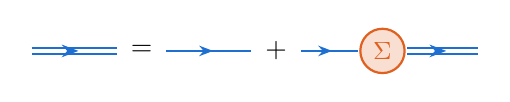
\begin{tikzpicture}[scale=0.9]
\draw[dfermion] (0,0)--(1.2,0); \node at (1.55,0) {$=$};
\draw[fermion] (1.9,0)--(3.1,0); \node at (3.45,0) {$+$};
\draw[fermion] (3.8,0)--(4.6,0); \node[sig] at (4.95,0) {$\Sigma$}; \draw[dfermion] (5.3,0)--(6.3,0);
\end{tikzpicture}
\vspace{0.2cm}
\begin{itemize}\small
 \item $\tauv\to\iw$: piecewise-linear interpolant integrated \emph{exactly} (no Gibbs ringing)
 \item $\iw\to\tauv$: subtract $c_1/\iw + c_2/(\iw)^2 + c_3/(\iw)^3$, FFT the rest, add the tail analytically
 \item tail coefficients fitted automatically (\texttt{tail\_coefficients})
\end{itemize}
\column{0.42\textwidth}
\begin{exampleblock}{Validated}
\small
\begin{itemize}
 \item $\tauv\leftrightarrow\iw$ round trip $<10^{-6}$
 \item free level: max error $<10^{-4}$
 \item density from $\G(\bet^-)$ to $10^{-8}$
\end{itemize}
\end{exampleblock}
\begin{block}{Grid}
\small \texttt{MatsubaraGrid(beta, n\_iw)} provides \texttt{iw}, \texttt{tau}, \texttt{tau\_to\_iw}, \texttt{iw\_to\_tau}, \texttt{density}.
\end{block}
\end{columns}
\end{frame}

% ======================================================================== 3
\section{Feynman diagrams}
\begin{frame}{Enumerating diagrams (Mattuck ch.\ 4, 9, 10)}
\begin{columns}[T]
\column{0.5\textwidth}
\begin{itemize}
 \item An order-$n$ diagram = permutation pairing $2n$ creation and annihilation points + $n$ interaction lines.
 \item Wick's theorem: sign $(-1)^{F}$ with $F$ = number of closed fermion loops.
 \item Connected, 1PI, skeleton (no $\Sig$ insertions) and Hartree (tadpole) filters.
 \item Counts reproduce Molinari's loop-resolved generating function, e.g.\ order 3: $10+9\ell+\ell^2$.
\end{itemize}
\begin{block}{Hubbard atom check}
\small Sum of the 12 fourth-order $\Sig$ diagrams $=0$: the exact $\Sig=\U^2/4\iw$ is purely second order. \ok
\end{block}
\column{0.47\textwidth}
\centering
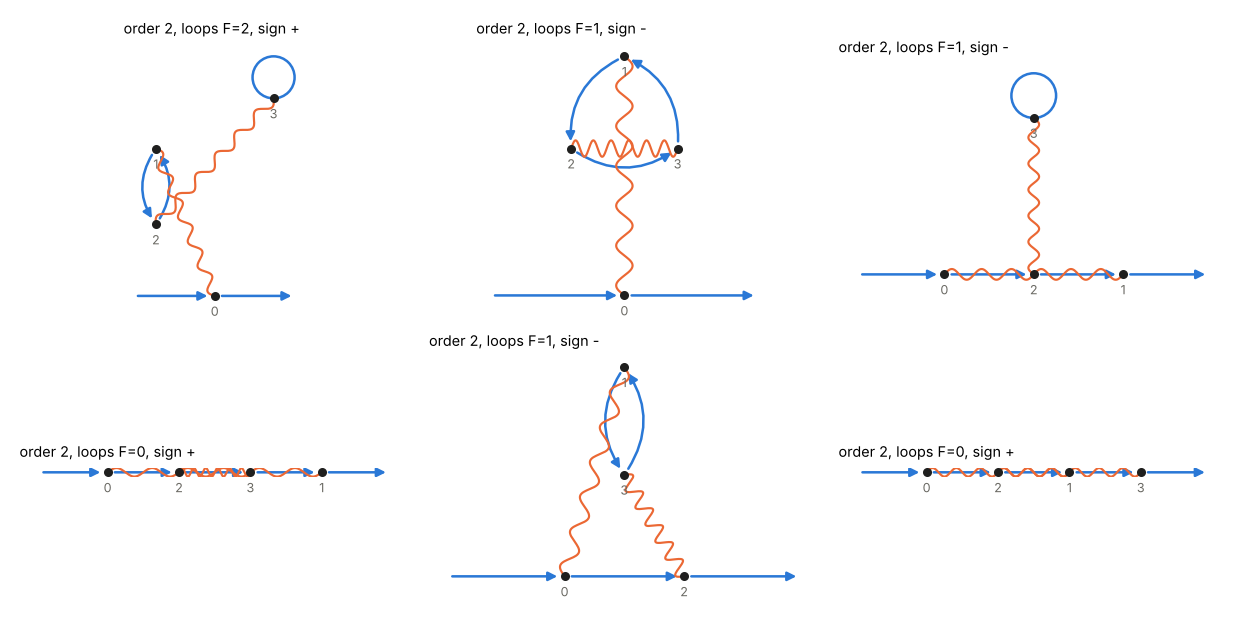
\includegraphics[width=\linewidth]{generic_sigma_order2.png}\\[2pt]
{\scriptsize second-order self-energy diagrams drawn by \texttt{diagrams.draw}}
\end{columns}
\end{frame}

\begin{frame}{Evaluating diagrams numerically}
\begin{columns}[T]
\column{0.52\textwidth}
Second-order self-energy (local, in imaginary time):
\[
\Sig^{(2)}(\tauv) = -\U^2\,\G(\tauv)\,\G(\tauv)\,\G(-\tauv)
\]
\centering
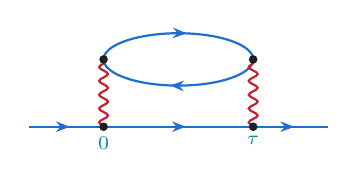
\begin{tikzpicture}[scale=0.95]
 \draw[fermion] (-2,0)--(-1,0); \draw[fermion] (-1,0)--(1,0); \draw[fermion] (1,0)--(2,0);
 \draw[fermion] (1,0.9) arc (0:-180:1 and 0.35);
 \draw[fermion] (-1,0.9) arc (180:0:1 and 0.35);
 \draw[inter] (-1,0)--(-1,0.9); \draw[inter] (1,0)--(1,0.9);
 \node[vtx] at (-1,0){}; \node[vtx] at (1,0){}; \node[vtx] at (-1,0.9){}; \node[vtx] at (1,0.9){};
 \node[below,font=\scriptsize\color{cT}] at (-1,0) {$0$}; \node[below,font=\scriptsize\color{cT}] at (1,0) {$\tau$};
\end{tikzpicture}
\begin{itemize}\small
 \item arbitrary diagrams: product of $\G(\tauv_i-\tauv_j)$ over lines, Monte Carlo over internal times
 \item exact for the Hubbard atom kernel and verified against second order to $10^{-10}$
\end{itemize}
\column{0.45\textwidth}
\centering
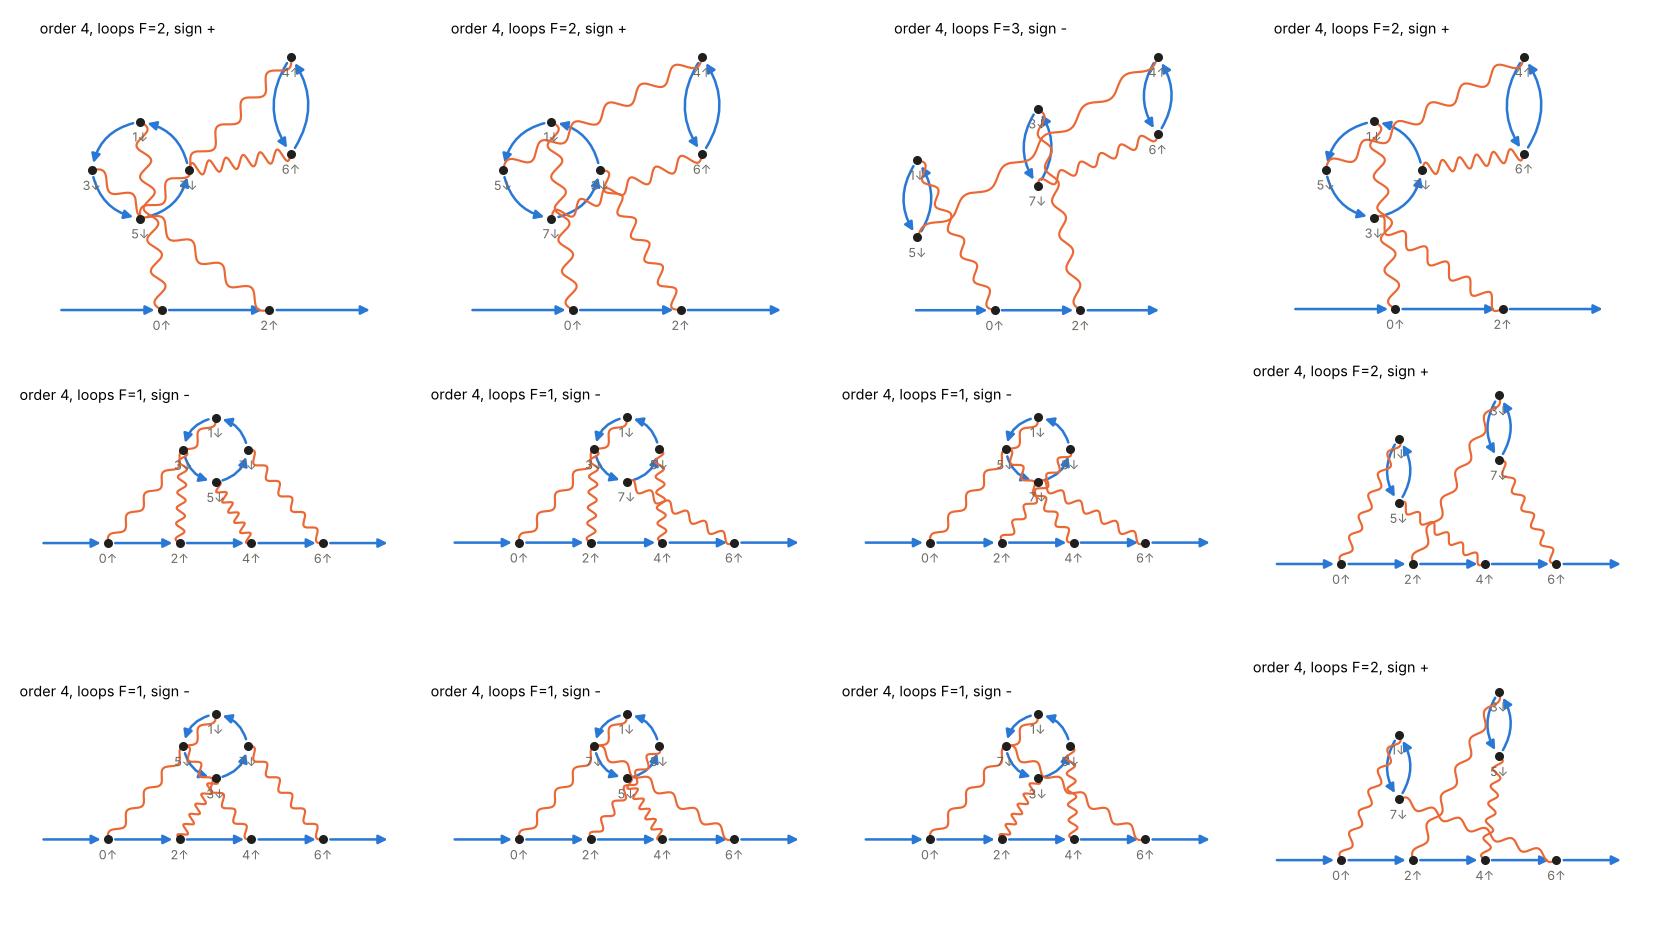
\includegraphics[width=\linewidth]{hubbard_sigma_order4.png}\\[2pt]
{\scriptsize fourth-order Hubbard-atom diagrams: the signs cancel exactly}
\end{columns}
\end{frame}

% ======================================================================== 4
\section{Self-energy: weak to strong coupling}
\begin{frame}{One interface, five approximations}
\renewcommand{\arraystretch}{1.3}
\small\begin{tabular}{p{2.3cm}p{5.8cm}p{4.9cm}}
\toprule
regime & approximation & benchmark \\ \midrule
weak $\U\ll W$ & 2nd order: $\Sig=\U^2\G\G\G$ & Yamada--Yosida $1/Z-1=(3-\pi^2/4)(\U/\pi\Gamma)^2$ \\
weak, collective & RPA / FLEX: $\Sig=\U^2\G\,\chiq/(1-\U\chiq)$ & Stoner $\U\chiq(\mathbf Q)=1$ detected \\
moderate & IPT (Georges--Kotliar) & coexistence $U_{c1}\!\approx\!2.5D$, $U_{c2}\!\approx\!3.3D$ \\
strong & Hubbard-I: atomic $\G$, $\Sig=\U^2/4\iw$ & atom exact \\
all & CT-INT / CT-HYB / ED / NRG & numerically exact \\
\bottomrule
\end{tabular}
\vspace{0.3cm}
\begin{alertblock}{Honest message}
IPT overestimates $U_{c2}$ (3.3D vs NRG 2.92--3.0D). feynlab flags such rows as \emph{informational} rather than ``passed''.
\end{alertblock}
\end{frame}

\begin{frame}{DMFT self-consistency and the Mott transition}
\begin{columns}[c]
\column{0.45\textwidth}
\centering
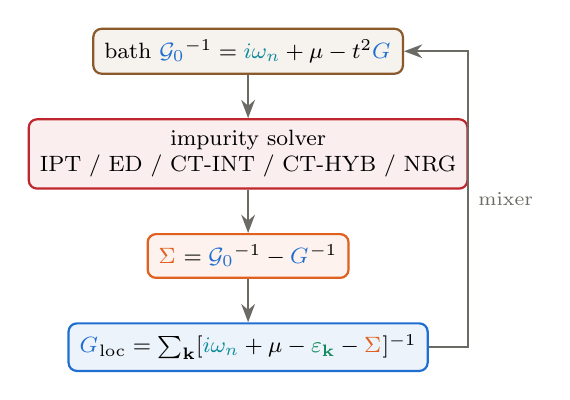
\begin{tikzpicture}[node distance=0.55cm]
\node[box=cD] (a) {bath $\Gw^{-1}=\iw+\mu-t^2\G$};
\node[box=cU,below=of a] (b) {impurity solver\\IPT / ED / CT-INT / CT-HYB / NRG};
\node[box=cS,below=of b] (c) {$\Sig=\Gw^{-1}-\G^{-1}$};
\node[box=cG,below=of c] (d) {$\G_{\rm loc}=\sum_{\mathbf k}[\iw+\mu-\ek-\Sig]^{-1}$};
\draw[-{Stealth},thick,muted] (a)--(b); \draw[-{Stealth},thick,muted] (b)--(c); \draw[-{Stealth},thick,muted] (c)--(d);
\draw[-{Stealth},thick,muted] (d.east) -- ++(0.5,0) |- node[pos=0.25,right,font=\scriptsize]{mixer} (a.east);
\end{tikzpicture}
\column{0.52\textwidth}
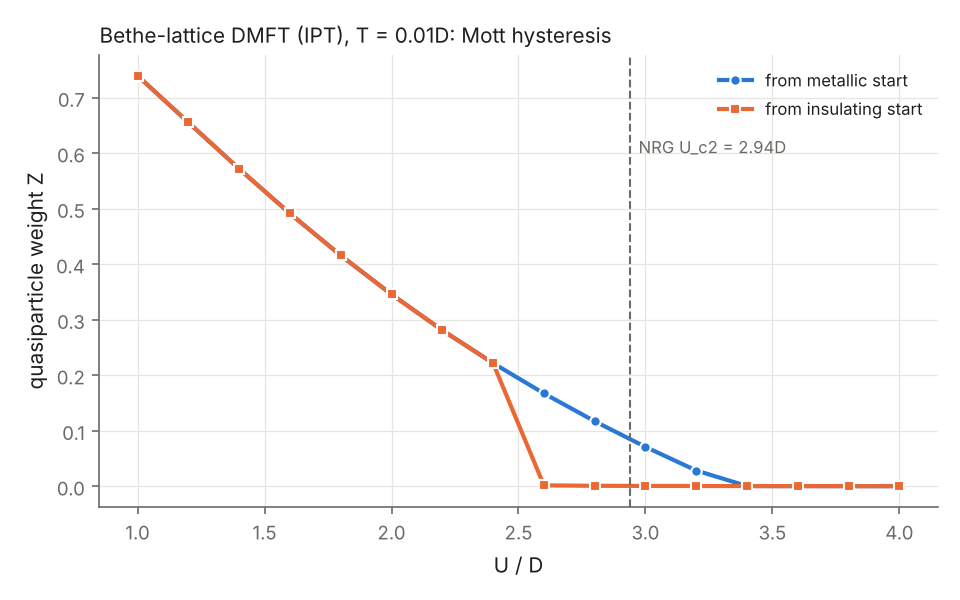
\includegraphics[width=\linewidth]{ipt_mott_hysteresis.png}
\end{columns}
\end{frame}

% ======================================================================== 5
\section{Quantum Monte Carlo}
\begin{frame}{CT-INT: weak-coupling continuous-time QMC}
\begin{columns}[c]
\column{0.5\textwidth}
\[
\frac{Z}{Z_0}=\sum_k \frac{(-\U)^k}{k!}\!\int\! d\tauv_1\!\ldots d\tauv_k
\]
\[
\times\prod_\sigma\det\big[\Gw^{\sigma}(\tauv_i-\tauv_j)-\alpha_{\sigma s_i}\delta_{ij}\big]
\]
\begin{itemize}\small
 \item one configuration = \emph{all} diagrams with the given vertices
 \item auxiliary shift $\delta\approx0.51$ removes the sign problem for $\U>0$
 \item fast updates $O(k^2)$; average order $\langle k\rangle\sim\bet\U$
 \item error bars from independent chains (+ $\Gamma$-method)
\end{itemize}
\column{0.47\textwidth}
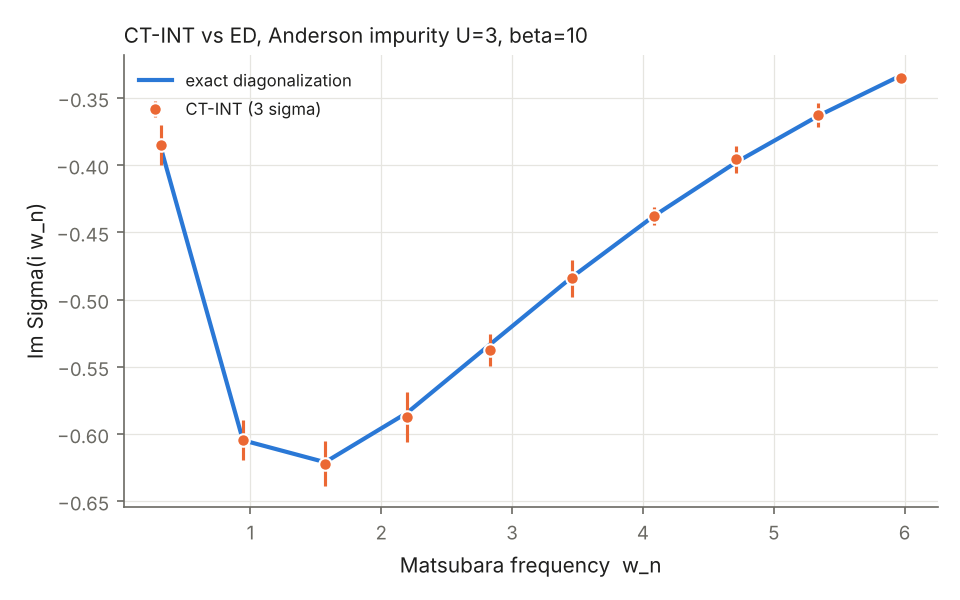
\includegraphics[width=\linewidth]{ctint_vs_ed.png}
\end{columns}
\end{frame}

\begin{frame}{CT-HYB: hybridization expansion in the segment picture \refcite{Werner et al.\ PRL 97, 076405 (2006)}}
\begin{columns}[T]
\column{0.53\textwidth}
\[
\frac{Z}{Z_{\rm bath}}=\sum_{k_\uparrow k_\downarrow}\int\!\prod_\sigma\det\big[{\color{cD}F_\sigma}(\tauv_i-\tauv'_j)\big]\,
e^{-\U\ell_{\rm ov}+\mu(\ell_\uparrow+\ell_\downarrow)}
\]
{\small ${\color{cD}F}(\tauv)=\Hyb(\bet-\tauv)$; average order \emph{decreases} with $\U$.}
\vspace{0.15cm}

\centering
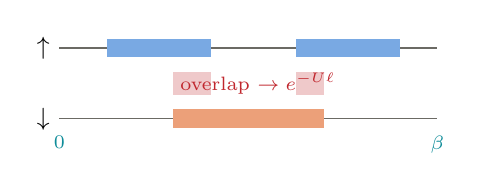
\begin{tikzpicture}[xscale=0.6]
\draw[muted] (0,0)--(8,0) (0,-0.9)--(8,-0.9);
\node[left,font=\small] at (0,0) {$\uparrow$}; \node[left,font=\small] at (0,-0.9) {$\downarrow$};
\fill[cG!60] (1,-0.12) rectangle (3.2,0.12); \fill[cG!60] (5.0,-0.12) rectangle (7.2,0.12);
\fill[cS!60] (2.4,-1.02) rectangle (5.6,-0.78);
\fill[cU!25] (2.4,-0.6) rectangle (3.2,-0.3); \fill[cU!25] (5.0,-0.6) rectangle (5.6,-0.3);
\node[font=\scriptsize,cU] at (4.2,-0.45) {overlap $\to e^{-U\ell}$};
\node[below,font=\scriptsize\color{cT}] at (0,-1.0) {$0$}; \node[below,font=\scriptsize\color{cT}] at (8,-1.0) {$\beta$};
\end{tikzpicture}
\begin{itemize}\small
 \item moves: insert/remove segment and anti-segment
 \item estimator $\G(\tauv)=-\frac1\bet\langle\sum M_{ji}\,\delta(\tauv-(\tauv_i-\tauv'_j))\rangle$
\end{itemize}
\column{0.44\textwidth}
\begin{exampleblock}{vs exact diagonalization ($\bet=10$)}
\small
\begin{tabular}{lcc}
 & CT-HYB & ED\\\midrule
$U=3$: $n_\sigma$ & 0.4713 & 0.4712\\
$U=3$: $\langle n_\uparrow n_\downarrow\rangle$ & 0.0828 & 0.0824\\
$U=4$: $\langle n_\uparrow n_\downarrow\rangle$ & 0.0780 & 0.0782\\
$U=4$: Im$\Sig(i\omega_0)$ & $-0.767$ & $-0.766$\\
\end{tabular}
\end{exampleblock}
\begin{block}{DMFT}
\small $U=2$, $\beta=20$: $Z=0.235$ (CT-HYB) vs 0.229 (finite-T ED-DMFT)
\end{block}
\end{columns}
\end{frame}

% ======================================================================== 6
\section{Exact diagonalization and the Mott transition}
\begin{frame}{Lanczos ED-DMFT at $T=0$}
\begin{columns}[T]
\column{0.5\textwidth}
\begin{itemize}\small
 \item sector-resolved sparse $\Ham$ ($N_\uparrow,N_\downarrow$ conserved)
 \item Lanczos ground state + continued fraction
 \[\G(z)=\frac{\langle d d^\dagger\rangle}{z-a_0-\frac{b_1^2}{z-a_1-\cdots}}+(\text{hole part})\]
 \item Caffarel--Krauth fit with \textbf{sum rule} $\sum_l V_l^2=\int\varepsilon^2\rho$, bounded levels, multi-start
\end{itemize}
\begin{alertblock}{Bath-parity effect}
\small odd bath $\Rightarrow$ singlet, zero mode $\Rightarrow$ use for $U_{c2}$;\\
even bath $\Rightarrow$ doublet $\Rightarrow$ use for $U_{c1}$
\end{alertblock}
\column{0.47\textwidth}
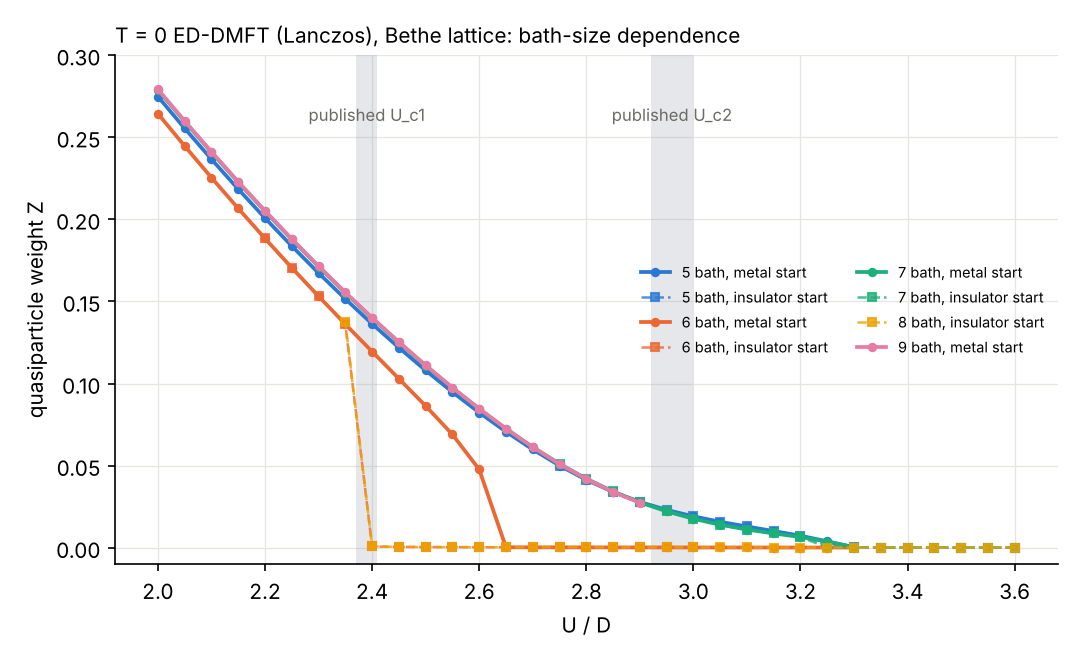
\includegraphics[width=\linewidth]{ed_dmft_mott_bath_size.png}\\
{\scriptsize consensus $U_{c1}=2.39D$, $U_{c2}=2.92$--$3.0D$ (NRG, DMRG)}
\end{columns}
\end{frame}

% ======================================================================== 7
\section{Multi-orbital, DFT+DMFT, DCA and NRG}
\begin{frame}{Kanamori interaction and Hund's physics}
\begin{columns}[c]
\column{0.53\textwidth}
\footnotesize
\begin{align*}
\Ham_{\rm int}&=\U\sum_a n_{a\uparrow}n_{a\downarrow}+{\color{cU}U'}\!\sum_{a\neq b}n_{a\uparrow}n_{b\downarrow}+({\color{cU}U'}-\J)\!\!\sum_{a<b,\sigma}\!n_{a\sigma}n_{b\sigma}\\
&-\J\!\sum_{a\neq b}c^\dagger_{a\uparrow}c_{a\downarrow}c^\dagger_{b\downarrow}c_{b\uparrow}+\J\!\sum_{a\neq b}c^\dagger_{a\uparrow}c^\dagger_{a\downarrow}c_{b\downarrow}c_{b\uparrow}\\
{\color{cU}U'}&=\U-2\J\quad\text{(rotational invariance)}
\end{align*}
\begin{itemize}\small
 \item \texttt{KanamoriAtom}: exact multiplets (sparse Jordan--Wigner)
 \item \texttt{MultiOrbitalED}: impurity solver $\le 8$ sites, one-orbital limit $=$ AndersonED to $10^{-14}$
 \item t$_{2g}^3$: $^4S$ at $3\U-9\J$, 4-fold \ok
\end{itemize}
\column{0.44\textwidth}
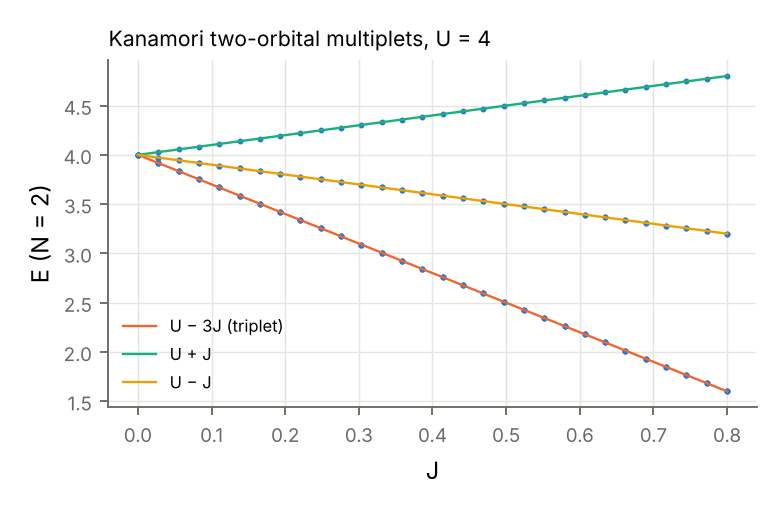
\includegraphics[width=\linewidth]{kanamori.png}
\end{columns}
\end{frame}

\begin{frame}{DFT+DMFT from Wannier90}
\begin{columns}[T]
\column{0.55\textwidth}
\[
\Ham(\mathbf k)=\sum_{\mathbf R}\frac{e^{i\mathbf k\cdot\mathbf R}}{\deg(\mathbf R)}\Ham_{\mathbf R}\quad(\texttt{seedname\_hr.dat})
\]
\[
\G_{\rm loc}(\iw)=\sum_{\mathbf k}\big[\iw+\mu-\Ham(\mathbf k)-P^\dagger(\Sig-\Sig_{\rm dc})P\big]^{-1}
\]
\begin{itemize}\small
 \item $\mu$ fixed to $n_{\rm elec}$ by bisection every iteration
 \item double counting: FLL $\U(n-\tfrac12)-\J(n_\sigma-\tfrac12)$, AMF, \emph{occupation} (plateau centre)
 \item solvers: Hubbard-I, multi-orbital ED
\end{itemize}
\column{0.42\textwidth}
\begin{exampleblock}{Checks}
\small
\begin{itemize}
 \item \texttt{hr.dat} write/read round trip exact
 \item $\U=0$: $Z=1$, $n=2.000000$
 \item $\U=4,\J=0.5$, half filling: Mott, $Z=0.0017$
\end{itemize}
\end{exampleblock}
\begin{block}{Not (yet)}
\small charge self-consistency; CT-HYB with full rotationally invariant $\J$
\end{block}
\end{columns}
\end{frame}

\begin{frame}{Dynamical cluster approximation and two-particle response}
\begin{columns}[T]
\column{0.5\textwidth}
\textbf{DCA} \refcite{Hettler et al.\ 1998; Maier et al.\ RMP 77, 1027 (2005)}
\[
\bar\G(\mathbf K)=\frac{N_c}{N}\sum_{\mathbf k\in\mathbf K}\frac{1}{\iw+\mu-\ek-\Sig(\mathbf K,\iw)}
\]
\begin{itemize}\small
 \item $N_c=1$: $Z=0.486644$ vs DMFT $0.486638$ \ok
 \item $N_c=4$: $Z(0,0)=0.565$, $Z(\pi,0)=0.475$ --- antinodal suppression
\end{itemize}
\column{0.47\textwidth}
\textbf{Two-particle}
\[
\chiq_0(\mathbf q,i\Omega)=-\frac{T}{N}\sum_{\mathbf k,\nu}\G(\mathbf k,i\nu)\G(\mathbf k+\mathbf q,i\nu+i\Omega)
\]
\[
\chiq_{s/c}=\frac{\chiq_0}{1\mp\U\chiq_0}
\]
\begin{itemize}\small
 \item compressibility sum rule $\chiq_0(0,0)=\partial n/\partial\mu$ to $10^{-8}$ \ok
 \item accepts dressed $\Sig$: first step to D$\Gamma$A
\end{itemize}
\end{columns}
\end{frame}

\begin{frame}{Numerical renormalization group and the Kondo effect}
\begin{columns}[c]
\column{0.4\textwidth}
\centering
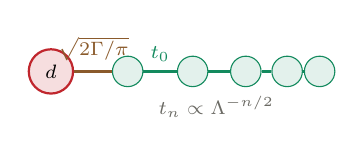
\begin{tikzpicture}[scale=0.75]
\node[circle,draw=cU,fill=cU!15,thick,minimum size=16pt,font=\scriptsize] (d) at (0,0) {$d$};
\foreach \i/\x in {0/1.3,1/2.4,2/3.3,3/4.0,4/4.55}{
  \node[circle,draw=cH,fill=cH!12,minimum size=11pt,inner sep=0] (c\i) at (\x,0) {};}
\draw[thick,cD] (d)--(c0) node[midway,above,font=\scriptsize]{$\sqrt{2\Gamma/\pi}$};
\draw[thick,cH] (c0)--(c1) node[midway,above,font=\scriptsize]{$t_0$};
\draw[thick,cH] (c1)--(c2); \draw[thick,cH] (c2)--(c3); \draw[thick,cH] (c3)--(c4);
\node[font=\scriptsize,muted] at (2.8,-0.6) {$t_n\propto\Lambda^{-n/2}$};
\end{tikzpicture}
\begin{itemize}\small
 \item log discretisation $\pm\Lambda^{-n}$, $A_\Lambda$ correction
 \item keep $N_{\rm keep}=300$--$400$ states, $\bar\beta=2$
 \item $U=0$: $S_{\rm imp}$ within 2--4\% of exact
 \item Haldane slope $-0.993$ (exact $-1$)
\end{itemize}
\column{0.57\textwidth}
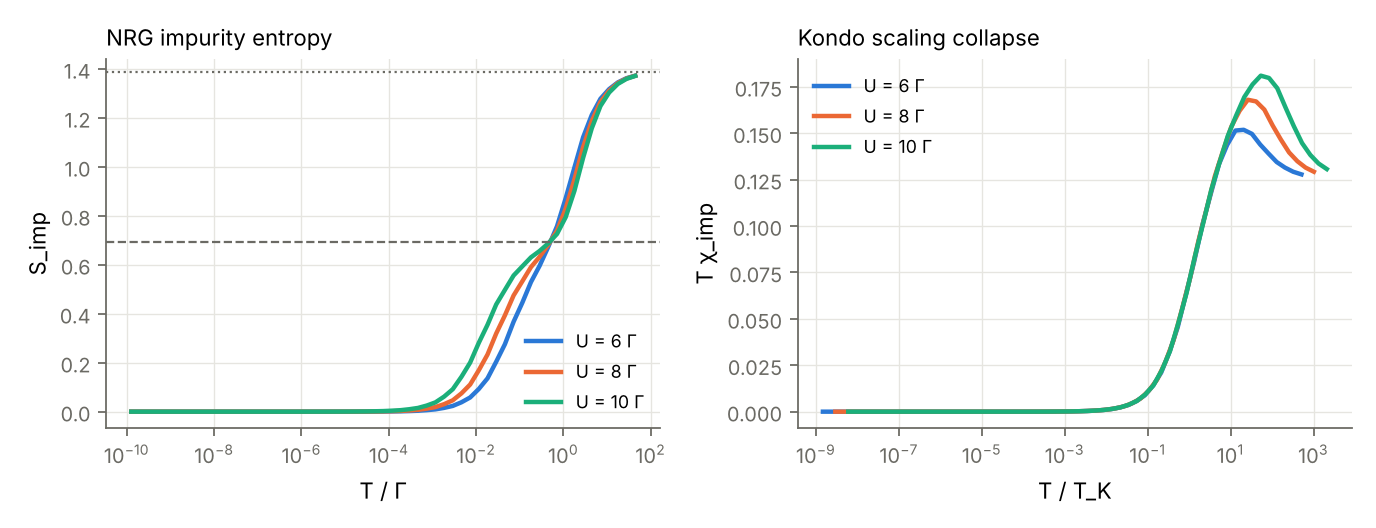
\includegraphics[width=\linewidth]{nrg_kondo.png}\\
{\scriptsize free orbital ($\ln4$) $\to$ local moment ($\ln2$) $\to$ Fermi liquid (0); universal collapse in $T/T_K$}
\end{columns}
\end{frame}

% ======================================================================== 8
\section{Analytic continuation}
\begin{frame}{From $\G(\iw)$ to $A(\omega)$: three complementary methods}
\begin{columns}[c]
\column{0.52\textwidth}
\[
\G(\iw)=\int d\omega\,\frac{A(\omega)}{\iw-\omega},\qquad A\ge0,\ \int A=1
\]
\renewcommand{\arraystretch}{1.25}
\small
\begin{tabular}{p{1.75cm}p{4.4cm}}
\toprule
MaxEnt & $\max_A\ \alpha S[A]-\chi^2/2$ \\
Nevanlinna & Schur interpolation of $h(-\G)$, exact causality; Pick test; 64-digit arithmetic \\
stochastic & average of $\delta$-function ensembles at $\chi^2/N\approx1$ \\
\bottomrule
\end{tabular}
\vspace{0.2cm}

\small Nevanlinna reproduces the input to $10^{-16}$ and continues off-axis exactly; normalisation 0.9955.
\column{0.45\textwidth}
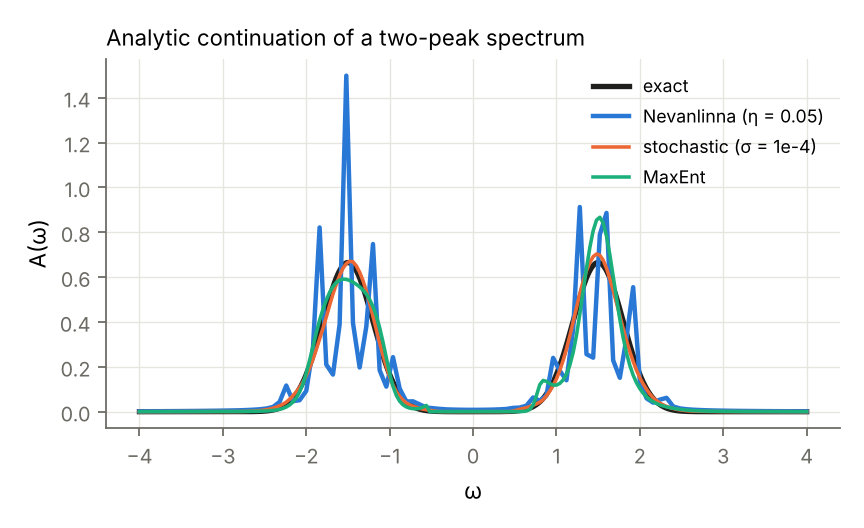
\includegraphics[width=\linewidth]{continuation.png}
\end{columns}
\end{frame}

% ======================================================================== 9
\section{Advanced diagrammatic Monte Carlo}
\begin{frame}{Connected determinants and resummation}
\begin{columns}[T]
\column{0.5\textwidth}
\textbf{CDet} \refcite{Rossi PRL 119, 045701 (2017)}
\[
c(V)=\det(V)-\!\!\sum_{S\subsetneq V,\,S\ni v_1}\! c(S)\,\det(V\setminus S)
\]
{\small all connected diagrams at cost $3^n$ (not $n!$)}
\begin{itemize}\small
 \item Hubbard atom: every Taylor coefficient of $-\tfrac14\tanh(\bet\U/4)$ \ok
 \item Anderson: $a_1=-0.06813$ vs ED $-0.06792$
\end{itemize}
\column{0.47\textwidth}
\textbf{Resummation}
\begin{itemize}\small
 \item Domb--Sykes: $R=1.0000$ for $(1+x)^{-1/2}$
 \item Pad\'e[8/8] at $x=3$: $0.50000001$
 \item conformal map at $x=3$: $0.4999999996$
\end{itemize}
\begin{alertblock}{Misleading convergence}
\small Skeleton series with exact $\G$ converges to the \textbf{wrong} $\Sig$ for $\bet\U\gtrsim5$ (Kozik--Ferrero--Georges 2015) --- reproduced; \texttt{misleading\_convergence\_check} flags it.
\end{alertblock}
\end{columns}
\end{frame}

\begin{frame}{Fr\"ohlich polaron: energy, $Z$ and $m^*$ by DiagMC}
\begin{columns}[T]
\column{0.55\textwidth}
\[
\G(p,\tauv)\xrightarrow{\tauv\to\infty} Z(p)\,e^{-[E(p)-\mu]\tauv}
\]
\begin{itemize}\small
 \item phonon arcs $\propto\alpha\,e^{-\tauv}/q^2$, momentum integrated analytically along the arc
 \item external momentum enters as $-\,\mathbf p\cdot\mathbf q\,\tauv$
 \item absolute $Z$ from the order-0 diagram $e^{-(p^2/2-\mu)\tauv}$ (known exactly)
 \item $m^*$ from $E(p)-E(0)=p^2/2m^*$
\end{itemize}
\column{0.42\textwidth}
\begin{exampleblock}{$\alpha=0.2$}
\small
\begin{tabular}{lcc}
 & DiagMC & weak coupling\\\midrule
$E$ & $-0.2015$ & $-0.2013$\\
$Z$ & $0.88$--$0.90$ & $1-\alpha/2=0.90$\\
$m^*/m$ & $1.05$--$1.08$ & $1.034$\\
\end{tabular}
\end{exampleblock}
{\scriptsize Mishchenko et al.\ PRB 62, 6317 (2000); R\"oseler 1968; Smondyrev 1986.\\ Statistical spread of $m^*$ is a few \% at $3\times10^7$ steps per chain.}
\end{columns}
\end{frame}

% ======================================================================== 10
\section{Hall transport: intrinsic and extrinsic}
\begin{frame}{Operator-resolved intrinsic Hall response}
\[
{\color{cX}\sigma^{O}_{xy}}=-e\sum_n\!\int\!\frac{d^2k}{(2\pi)^2}f_n\,{\color{cB}\Omega^{O}_n},\qquad
{\color{cB}\Omega^O_n}=-2\,\mathrm{Im}\sum_{m\neq n}\frac{\langle n|\jcur{O}_x|m\rangle\langle m|\vel{y}|n\rangle}{(E_n-E_m)^2},\qquad
\jcur{O}_x=\tfrac12\{\Op,\vel{x}\}
\]
\begin{columns}[T]
\column{0.5\textwidth}
\begin{itemize}\small
 \item $\Op=1$: AHE (TKNN); $S_z$: SHC; $L_z$: OHC; $Q_{ab}$: orbital-quadrupole Hall
 \item Chern numbers by Fukui--Hatsugai--Suzuki (integers on any grid)
 \item models: massive Dirac, Rashba, QWZ, Haldane, $p$-orbital square, Wannier TB (2D/3D)
\end{itemize}
\column{0.47\textwidth}
\begin{exampleblock}{Checks}
\small
\begin{itemize}
 \item QWZ/Haldane: $\sxy=-C$ exactly
 \item Rashba SHC $=e/8\pi$ (Sinova 2004)
 \item Dirac $\sigma_{\rm int}=-\Delta/2\mu$ (Sinitsyn 2007)
\end{itemize}
\end{exampleblock}
\end{columns}
\end{frame}

\begin{frame}{Kubo--St\v{r}eda with disorder: side jump and skew scattering}
\begin{columns}[c]
\column{0.52\textwidth}
\[
{\color{cX}\sigma^{I}_{xy}}=\frac{1}{2\pi}\int\frac{d^2k}{(2\pi)^2}\mathrm{Tr}\big[\jcur{O}_x\G^R\,{\color{cV}\Gamma_y}\,\G^A\big]
\]
\[
{\color{cV}\Gamma_y}=\vel{y}+n_i\Vimp^2\!\int\!\G^A{\color{cV}\Gamma_y}\G^R+n_i{\color{cU}V_1^3}(\ldots)
\]
\begin{itemize}\small
 \item Born $\Sig$, ladder vertex, third-order skew vertex
 \item decomposition intrinsic / side jump / anomalous distribution / intrinsic skew / extrinsic skew
 \item Dirac model: all terms reproduce Sinitsyn et al.\ PRB 75, 045315 to $10^{-3}$
 \item Rashba: SHC vertex cancellation $e/8\pi-e/8\pi=0$ (Inoue 2004) \ok
\end{itemize}
\column{0.45\textwidth}
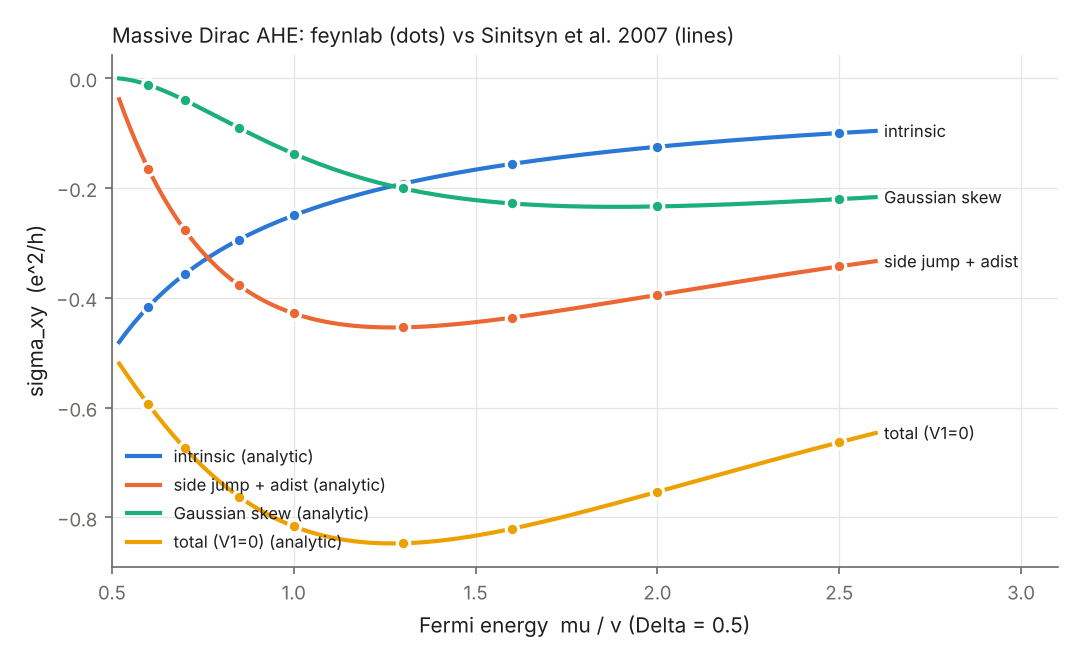
\includegraphics[width=\linewidth]{ahe_dirac_mechanisms.png}
\end{columns}
\end{frame}

\begin{frame}{Crossed X and $\Psi$ diagrams \refcite{Ado, Dmitriev, Ostrovsky, Titov EPL 111, 37004 (2015)}}
\begin{columns}[T]
\column{0.48\textwidth}
\centering
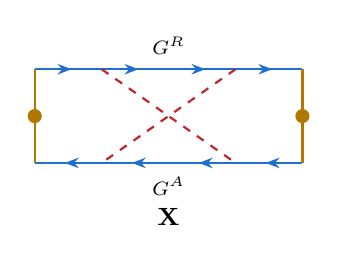
\begin{tikzpicture}[scale=0.85]
\draw[fermion] (0,0)--(1,0); \draw[fermion] (1,0)--(2,0); \draw[fermion] (2,0)--(3,0); \draw[fermion] (3,0)--(4,0);
\draw[fermion] (4,-1.4)--(3,-1.4); \draw[fermion] (3,-1.4)--(2,-1.4); \draw[fermion] (2,-1.4)--(1,-1.4); \draw[fermion] (1,-1.4)--(0,-1.4);
\draw[imp] (1,0)--(3,-1.4); \draw[imp] (3,0)--(1,-1.4);
\fill[cV] (0,-0.7) circle (3pt); \fill[cV] (4,-0.7) circle (3pt);
\draw[thick,cV] (0,0)--(0,-1.4); \draw[thick,cV] (4,0)--(4,-1.4);
\node[font=\scriptsize] at (2,0.35) {$G^R$}; \node[font=\scriptsize] at (2,-1.75) {$G^A$};
\node[font=\small\bfseries] at (2,-2.2) {X};
\end{tikzpicture}
\hspace{0.3cm}
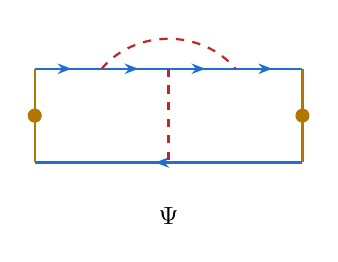
\begin{tikzpicture}[scale=0.85]
\draw[fermion] (0,0)--(1,0); \draw[fermion] (1,0)--(2,0); \draw[fermion] (2,0)--(3,0); \draw[fermion] (3,0)--(4,0);
\draw[fermion] (4,-1.4)--(0,-1.4);
\draw[imp] (1,0) to[bend left=50] (3,0); \draw[imp] (2,0)--(2,-1.4);
\fill[cV] (0,-0.7) circle (3pt); \fill[cV] (4,-0.7) circle (3pt);
\draw[thick,cV] (0,0)--(0,-1.4); \draw[thick,cV] (4,0)--(4,-1.4);
\node[font=\small\bfseries] at (2,-2.2) {$\Psi$};
\end{tikzpicture}
\vspace{0.1cm}

{\small skew scattering on \emph{pairs} of close impurities; same order as side jump}
\column{0.5\textwidth}
\begin{itemize}\small
 \item real-space evaluation with FFTs, dressed vertices, extrapolation $\Gamma\to0$
 \item continuum Dirac: $X=4\varepsilon m(\varepsilon^2-m^2)/(\varepsilon^2+3m^2)^2$ within 1.5\%, $\Psi=0$ \ok
 \item \textbf{v1.0: lattice version} (FFT over the BZ)
\end{itemize}
\begin{exampleblock}{QWZ ($m=-1.7$) vs $k\!\cdot\!p$ limit}
\small
\begin{tabular}{lcc}
 & lattice & $\Delta-k^2/2$ continuum\\\midrule
$X$ & 0.795 & 0.790\\
$\Psi$ & $-0.499$ & $-0.524$\\
\end{tabular}\\[2pt]
$\Psi\neq0$: generated by the quadratic mass of real bands.
\end{exampleblock}
\end{columns}
\end{frame}

\begin{frame}{Beyond scalar Gaussian disorder}
\framesubtitle{matrix impurities and the self-consistent T-matrix}
\begin{columns}[T]
\column{0.5\textwidth}
\textbf{Matrix impurities} $V_{\rm imp}=\Vimp M$\\
{\small ($M=\sigma_z$, orbital projector, $L_z$, \ldots)}
\[
\Sig=n_i\Vimp^2\, M\bar g M^\dagger,\qquad \text{rung: } n_i\Vimp^2\, M\otimes M^*
\]
\textbf{Self-consistent T-matrix}
\[
\Tm=\Vimp(1-\bar g\Vimp)^{-1},\qquad \Sig=n_i(\Tm-\Vimp)
\]
\[
\text{rung: } n_i\,\Tm^R\otimes\Tm^A
\]
{\small Third order: $n_i\Vimp^3\bar g$ $\Rightarrow$ skew scattering appears automatically.}
\column{0.47\textwidth}
\begin{exampleblock}{Checks (Dirac, $\mu=1$, $n_i\Vimp^2=0.005$)}
\small
\begin{tabular}{p{3.6cm}r}
$M=\mathbb 1$ vs scalar & identical\\
T-matrix vs Born + skew ($V_1=\Vimp$) & $1.4\times10^{-4}$\\
$\Vimp=\pm0.5$: even part / Born & 0.989\\
\end{tabular}
\end{exampleblock}
{\small Use cases: resonant (unitary) scatterers, magnetic impurities, orbital-selective disorder for orbital Hall transport.}
\end{columns}
\end{frame}

% ======================================================================== 11
\section{Orbitronics toolbox}
\begin{frame}{Orbital moment, BCD, Edelstein effect, finite temperature}
\begin{columns}[c]
\column{0.44\textwidth}
\small
\[
\morb_n(\mathbf k)=\mathrm{Im}\sum_{m\neq n}\frac{\vel{x}_{nm}\vel{y}_{mn}}{E_n-E_m}
\]
\[
\Dip_a=\sum_n\!\int f_n\,\partial_a\Om_n=\sum_n\!\int(-f')\,\vel{a}_{nn}\Om_n
\]
\[
\delta\langle\Op\rangle=-e E\tau\sum_n\!\int(-f')\,\vel{x}_{nn}\Op_{nn}
\]
\[
{\color{cX}\sigma}(\mu,T)=\int dE\,(-f')\,{\color{cX}\sigma}(E,0)
\]
\begin{itemize}\scriptsize
 \item valley moment = Xiao--Yao--Niu to $10^{-15}$
 \item BCD sea $=$ surface to $10^{-8}$; $D=0$ without tilt
 \item Rashba $|\delta S_y|=m\alpha/4\pi$ to $10^{-4}$
 \item Kubo odd part $=$ Boltzmann; even (intrinsic SOT) part $=0$ without magnetisation
\end{itemize}
\column{0.54\textwidth}
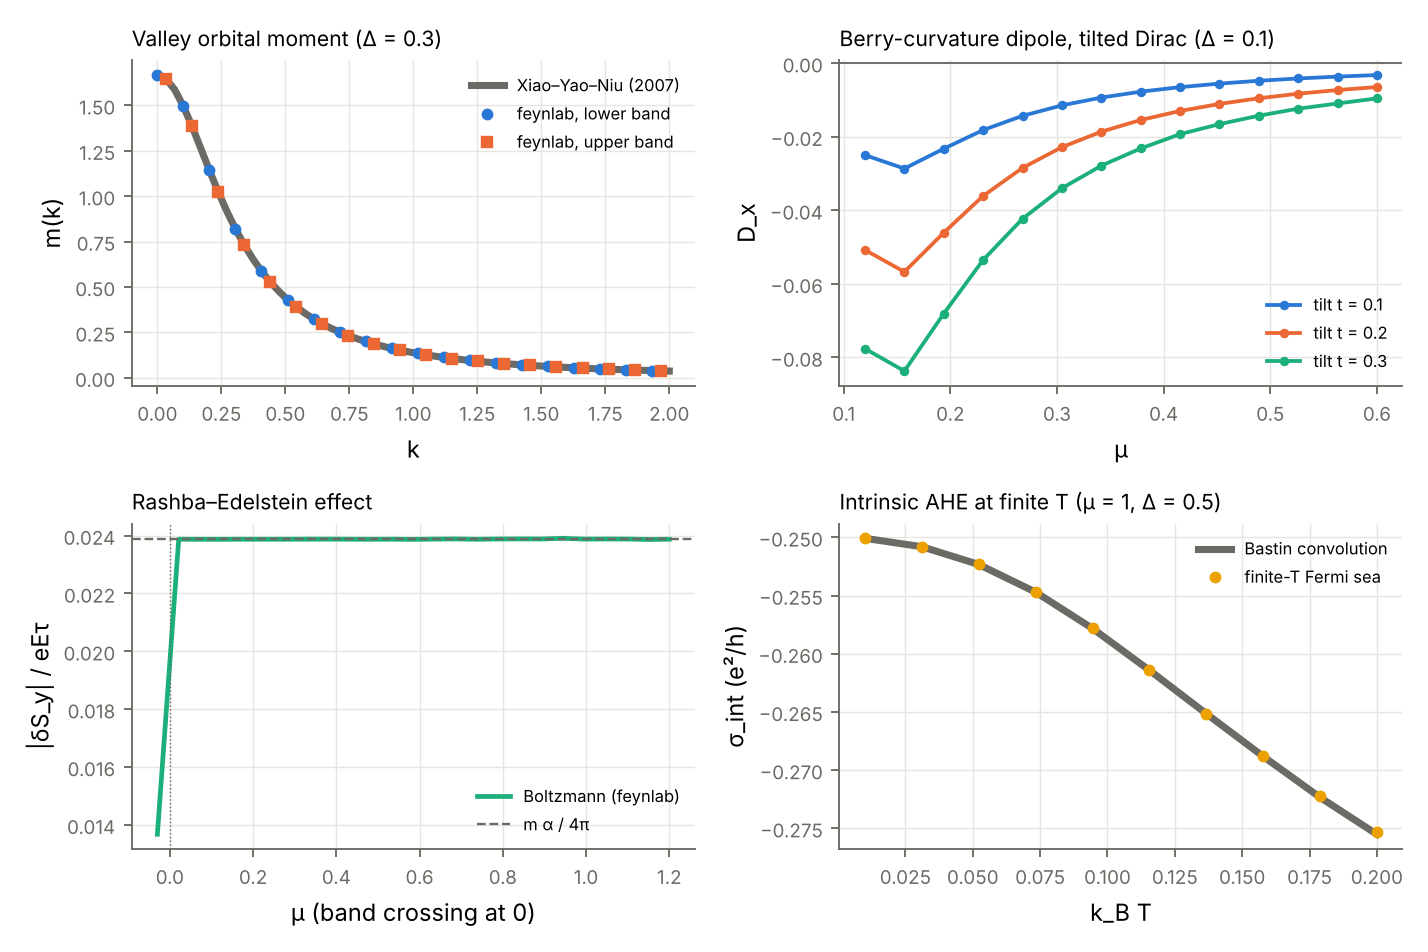
\includegraphics[width=\linewidth]{transport_v1.png}
\end{columns}
\end{frame}

\begin{frame}{Three-dimensional Wannier Hall tensors with adaptive refinement}
\begin{columns}[T]
\column{0.53\textwidth}
\[
{\color{cX}\sigma_c}=-\frac{2\pi}{V_{\rm cell}}\Big\langle\sum_n f_n\,{\color{cB}\Omega_{n,c}}\Big\rangle_{\rm BZ},\quad c\leftrightarrow(yz,zx,xy)
\]
\begin{itemize}\small
 \item reads any \texttt{seedname\_hr.dat} + lattice vectors (\AA)
 \item operator-resolved: \texttt{op=Sz} (SHC), \texttt{op=Lz} (OHC)
 \item refine cells with large $|\Om|$ \emph{or} a band within a window of $\mu$ by $n_{\rm sub}^3$ sub-meshes \refcite{Wang, Yates, Souza, Vanderbilt PRB 74, 195118 (2006)}
 \item output in $(e^2/h)/$\AA\ and S/cm
\end{itemize}
\column{0.44\textwidth}
\begin{exampleblock}{Stacked Chern layers ($c=3$\,\AA)}
\small $\sxy=C\,e^2/hc$ reproduced to $10^{-7}$ (Halperin 1987)
\end{exampleblock}
\begin{exampleblock}{Metallic case, $\mu=-0.9$}
\small
\begin{tabular}{lc}
mesh & $\sxy$\\\midrule
plain $40^3$ & 0.21178 (0.6\%)\\
adaptive $40^3$ & 0.21006 (0.2\%)\\
converged $200^2\times160$ & 0.21040\\
\end{tabular}
\end{exampleblock}
\end{columns}
\end{frame}

% ======================================================================== 12
\section{Robustness and engineering}
\begin{frame}{Error analysis, mixing, checkpoints}
\begin{columns}[c]
\column{0.52\textwidth}
\begin{itemize}\small
 \item \textbf{$\Gamma$-method} (Wolff 2004): $\tau_{\rm int}=9.0$ vs exact 9.5 for AR(1), $\phi=0.9$
 \item binning analysis, jackknife for derived quantities
 \item \textbf{Anderson / Broyden} mixing: IPT at $U=2.6$ converges in 13 / 12 iterations instead of 78; identical fixed point to $10^{-10}$
 \item \textbf{HDF5 checkpoints}: restart any DMFT loop
 \item \textbf{CLI}: \texttt{feynlab dmft|hall|polaron|nrg input.toml}; inputs stored in output
 \item \textbf{GPU}: optional CuPy backend; \textbf{units} layer (eV, \AA, S/cm)
 \item \textbf{CI}: tests on push, full benchmarks weekly; CITATION.cff, Zenodo DOI, MkDocs site
\end{itemize}
\column{0.45\textwidth}
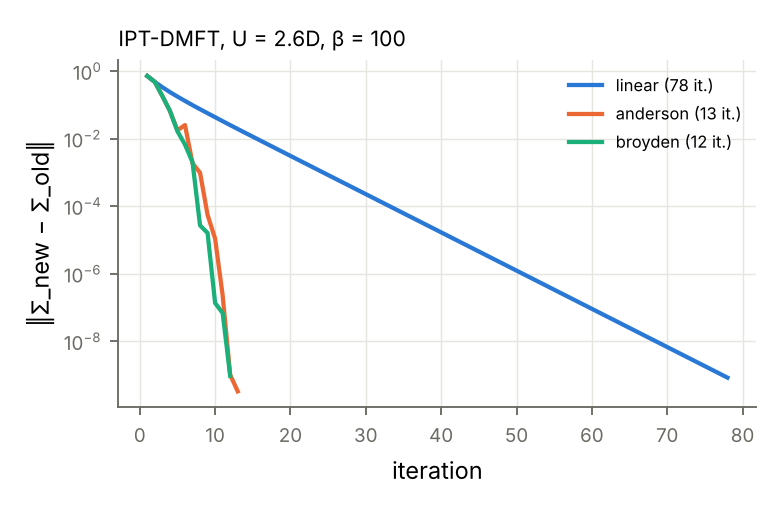
\includegraphics[width=\linewidth]{mixers.png}
\end{columns}
\end{frame}

% ======================================================================== v1.1
\section{v1.1: closing every v1.0 limitation}
\begin{frame}{From limitation to validated feature}
\scriptsize
\renewcommand{\arraystretch}{1.12}
\begin{tabular}{p{3.9cm}p{5.3cm}p{4.0cm}}
\toprule
v1.0 limitation & v1.1 implementation & validation\\\midrule
CT-HYB density--density only & matrix CT-HYB, full local trace & 2-orbital Kanamori ED, $1\sigma$\\
DCA solver 2nd order & cluster CT-INT (exact) & dimer+bath ED, $1\sigma$\\
no charge self-consistency & $H(\mathbf k)=H_0+V[n]$, $N(\mathbf k)$ export & Hartree mean field $6\times10^{-6}$\\
two-particle = RPA & ED vertex, BSE, DMFT $\chiq(\mathbf q)$, ladder D$\Gamma$A, TPSC & $\chi_m(0)=dm/dh$ to 0.04\%\\
Nevanlinna, no Hardy & Hardy-basis optimisation, dps $=3n$ & L1 $0.04$--$0.06$ (raw $\sim1$)\\
stochastic $<$ MaxEnt & SAC, Shao--Sandvik criterion & L1 0.075 vs 0.25\\
polaron $m^*$ $\pm$few\% & momentum-fluctuation estimator & $1.0340\pm0.0002$ (1.0343)\\
semiclassical Gaussian skew & complete $w^{(4a)}$ (factor-2 slip found) & Sinitsyn $10^{-6}$\\
$\delta$-correlated disorder & finite-range impurities & Bessel formula $10^{-10}$\\
crossed diagrams: square only & any 2D/3D Bravais lattice & oblique cell, 3D stacks\\
no lattice polarons & Holstein / SSH variational ED & $E_0=-2.46968472393287$\\
chains serial & MPI / process pool & identical results\\
\bottomrule
\end{tabular}
\end{frame}

\begin{frame}{Matrix CT-HYB: the full Kanamori interaction}
\begin{columns}[T]
\column{0.55\textwidth}
{\small
\[
w(C)=\prod_f\det F_f\;\, s_P\,\mathrm{Tr}\Big[\prod_{i}^{\leftarrow} e^{-(t_{i-1}-t_i)\Ham}\,O_i\Big]e^{-t_K\Ham}
\]}
{\small ${\color{cD}F}(\tauv)=-\Hyb(\bet-\tauv)$; $s_P$ = parity of time ordering; operators in the eigenbasis of $\Ham_{\rm loc}$}
\begin{itemize}\small
 \item spin flip and pair hopping exact; observables by operator insertion
 \item inside DFT+DMFT: noise-aware frequency cut-off + Kanamori HF tail $\Sig_\infty$
\end{itemize}
\begin{alertblock}{Two bugs found by the ED comparison}
\small (i) \texttt{continue} on impossible moves skipped measurements $\Rightarrow$ $\G$ +10\%;\;
(ii) stale operator ordering after a rejected removal $\Rightarrow$ sign 0.77.
\end{alertblock}
\column{0.42\textwidth}
\begin{exampleblock}{2 orbitals, $U=2.5$, $J=0.4$, $\beta=5$}
\small
\begin{tabular}{lcc}
 & CT-HYB & ED\\\midrule
$n_{0\uparrow}$ & 0.4983(5) & 0.4988\\
$\langle n_\uparrow n_\downarrow\rangle_0$ & 0.0942(5) & 0.0944\\
$n_{1\uparrow}$ & 0.4465(11) & 0.4460\\
$\langle S_z^2\rangle$ & 0.4810(5) & 0.4810\\
sign & 1 & --\\
\end{tabular}
\end{exampleblock}
{\small one-band lattice DMFT: $Z=0.250$ (matrix) vs $0.247$ (segment)}
\end{columns}
\end{frame}

\begin{frame}{Cluster CT-INT, exact DCA and charge self-consistency}
\begin{columns}[T]
\column{0.5\textwidth}
\textbf{Cluster CT-INT}
\[
D_\sigma[p,q]=\tilde{\Gw}(\mathbf r_p-\mathbf r_q,\tauv_p-\tauv_q)-\alpha_\sigma(s_p)\delta_{pq}
\]
\[
\G(\mathbf K)=\tilde{\Gw}(\mathbf K)-\tilde{\Gw}(\mathbf K)^2S(\mathbf K,\iw)/\bet
\]
\begin{itemize}\scriptsize
 \item dimer in a bath: $\Sig(\mathbf K,i\omega_0)$ vs ED within $1\sigma$ ($K=0,\pi$)
 \item DCA $N_c=1$: $Z=0.4721$ vs single-site CT-INT $0.4709$
\end{itemize}
\column{0.47\textwidth}
\textbf{Charge self-consistency}
\[
N_{ab}(\mathbf k)=T\sum_n\G_{ab}(\mathbf k,\iw)e^{\iw0^+}
\]
\[
\Ham(\mathbf k)=\Ham_0(\mathbf k)+V[n]
\]
\begin{itemize}\scriptsize
 \item $N(\mathbf k)$ exact to $3\times10^{-7}$ at $U=0$ (analytic $1/(i\omega)^2$ tail)
 \item $U_{\rm DMFT}=0$: CSC $\equiv$ Hartree mean field ($6\times10^{-6}$)
 \item electron count now uses $c_2=\langle\Ham\rangle-\mu+\mathrm{Re}\Sig(i\infty)$ (was 1.2\% off)
 \item \texttt{write\_density\_matrix} for an external DFT code
\end{itemize}
\end{columns}
\end{frame}

\begin{frame}{Two-particle vertex, DMFT susceptibility, ladder D$\Gamma$A, TPSC}
\begin{columns}[T]
\column{0.53\textwidth}
\small
\[
\int_{\beta>t_a>t_b>t_c>0}\!\!\!\!e^{\sum x t}=f[0,x_a,x_a{+}x_b,x_a{+}x_b{+}x_c]
\]
{\scriptsize divided differences via $\exp(\beta J)$, $J$ bidiagonal: stable for degenerate levels}
\[
\chiq_r(\mathbf q)^{-1}=\chiq_0(\mathbf q)^{-1}+\Gamma_r/\bet^2,\quad r=d,m
\]
{\footnotesize
\begin{align*}
\Sig_{\rm D\Gamma A}&=\Sig_{\rm DMFT}-\frac{\U}{\bet^2}\sum_{\mathbf q\omega\nu'}K(\mathbf q)\,\G\G\G\;-\;(\text{local})\\
K(\mathbf q)&=\tfrac12F_d(\mathbf q)-\tfrac32F_m(\mathbf q)-\tfrac12F_d^{\rm loc}+\tfrac12F_m^{\rm loc}\;\xrightarrow{U\to0}\;\U
\end{align*}}
\column{0.44\textwidth}
\begin{exampleblock}{Checks}
\scriptsize
\begin{itemize}
 \item Wick ($U=0$): $10^{-15}$
 \item Schwinger--Dyson with ED $F_{\uparrow\downarrow}$ = ED $\Sig$ (0.05\%)
 \item DMFT $\chi_m(\mathbf q{=}0)$: BSE 2.9089 vs $dm/dh$ 2.9102
 \item D$\Gamma$A $\to$ 2nd order as $U\to0$ (deviation $\propto U$)
 \item TPSC: both sum rules exact; $\mathrm{Tr}\,\Sig G^0=U\langle n_\uparrow n_\downarrow\rangle$ ($1/N\to0$)
\end{itemize}
\end{exampleblock}
\end{columns}
\end{frame}

\begin{frame}{Transport closures: Gaussian skew from rates, smooth disorder, generic crossed diagrams}
\begin{columns}[c]
\column{0.42\textwidth}
\small
\begin{itemize}
 \item $w^{(4a)}$: $T_1T_3^*$ (on-shell $\Sig$ $\times$ interband $\G$) $+\ |T_2|^2$ interference
 \item Dirac: Sinitsyn to $10^{-6}$; quadratic-mass Dirac: Kubo residual to $10^{-4}$
 \item the v1.0 ``missing half'' was a transcription factor 2
 \item finite range $u(q)=e^{-q^2d^2/4}$: $\sigma_{xx}$ = Bessel formula; side jump suppressed by smooth disorder
 \item \texttt{LatticeCrossed}: any Bravais lattice, 2D/3D, $\Op=S_z,L_z$
\end{itemize}
\column{0.56\textwidth}
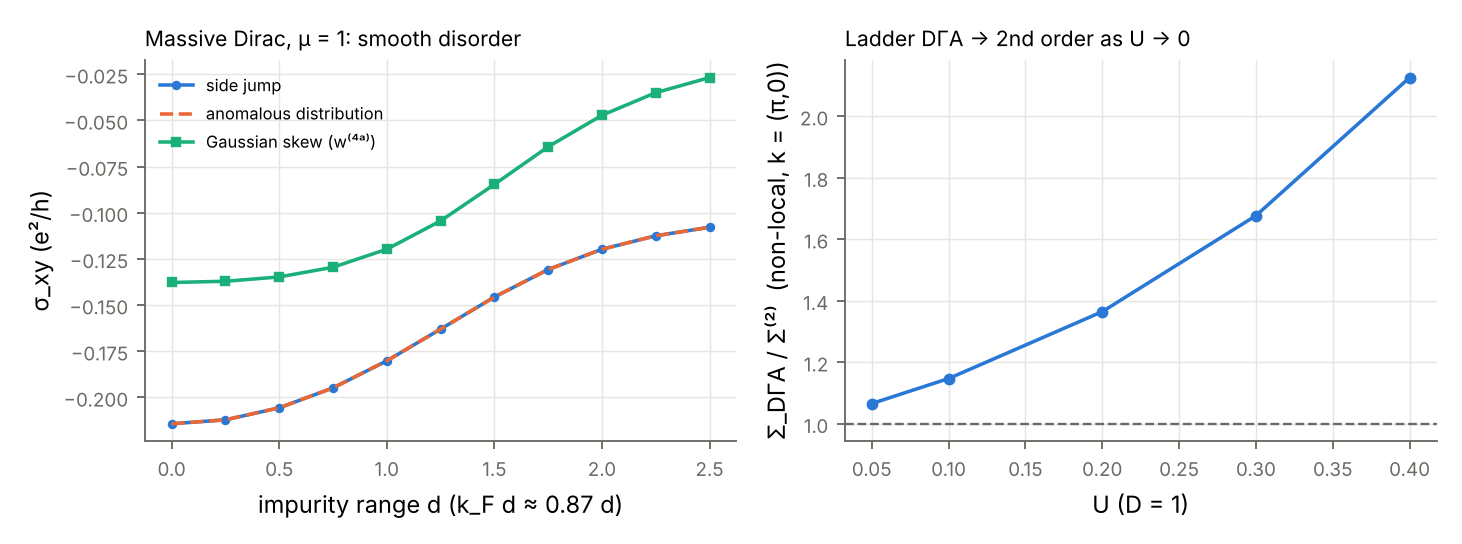
\includegraphics[width=\linewidth]{transport_dga_v11.png}
\end{columns}
\end{frame}

\begin{frame}{Continuation and polarons, upgraded}
\begin{columns}[c]
\column{0.56\textwidth}
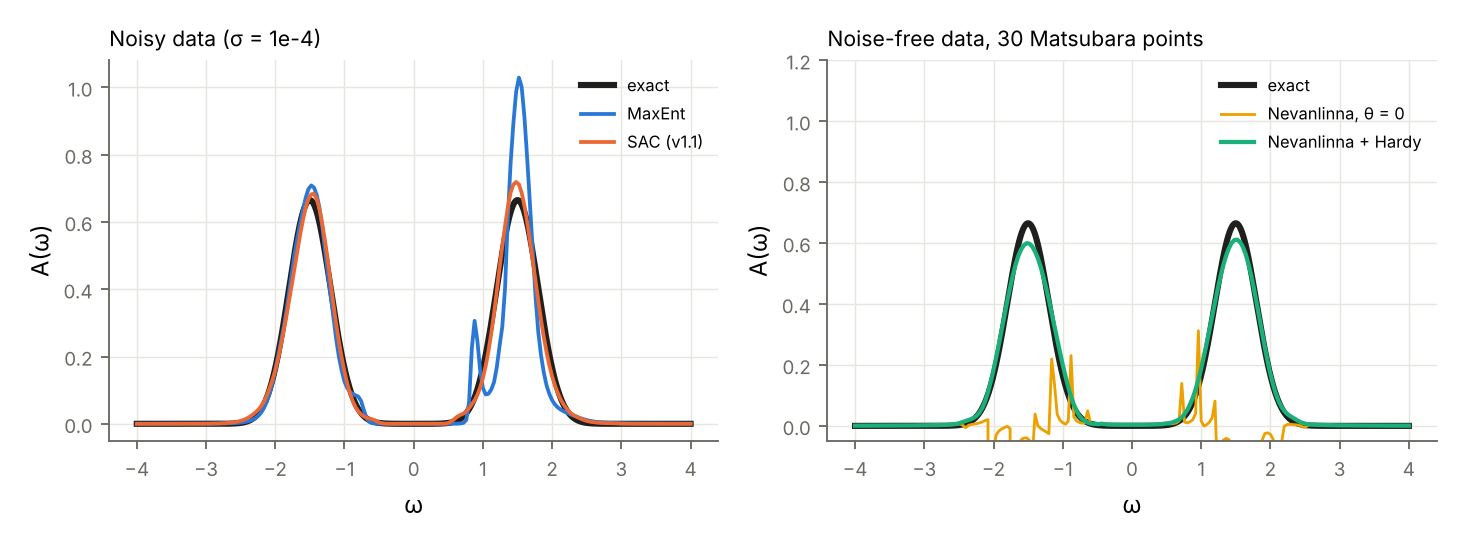
\includegraphics[width=\linewidth]{continuation_v11.png}\\[2pt]
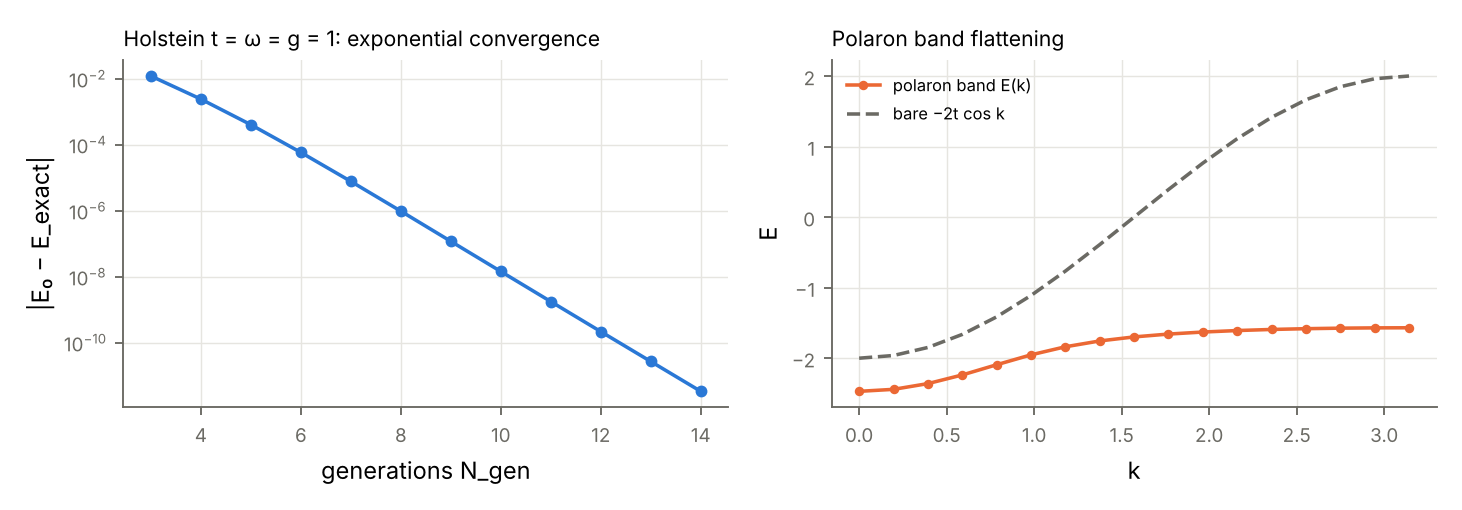
\includegraphics[width=\linewidth]{holstein_v11.png}
\column{0.41\textwidth}
\small
\begin{itemize}
 \item SAC: L1 0.075 (MaxEnt 0.25)
 \item Nevanlinna + Hardy: L1 0.04--0.06
 \item Fr\"ohlich $m^*$: \[\frac{m}{m^*}=1-\lim_{\tau\to\infty}\frac{\langle X^2\rangle}{3\tau},\ X=\sum q\,(t_2-t_1)\]
 \item Holstein $E_0=-2.46968472393287$ (published 21-digit value)
\end{itemize}
\end{columns}
\end{frame}

% ======================================================================== 13
\section{v1.2: first-principles charge self-consistency}
\begin{frame}{DFT+DMFT with QE + Wannier90 \refcite{Beck et al., JPCM 34, 235601 (2022)}}
\begin{columns}[T]
\column{0.53\textwidth}
\small
\textbf{Cycle} (\texttt{feynlab.dft.qe\_csc.QEDMFT})
\begin{enumerate}\footnotesize
 \item \texttt{pw.x} scf $\to$ nscf (\texttt{dmft=.true.}) $\to$ Wannier90 $U(\mathbf k)$
 \item $\Ham_W(\mathbf k)=V^\dagger\,\mathrm{diag}(\ek)\,V$, \;DMFT $\to\Sig$
 \item window density matrix
 \[N(\mathbf k)=\tfrac1{\bet}\textstyle\sum_n\big[\iw+\mu-\ek-V(\Sig-\Sig[dc])V^\dagger\big]^{-1}\]
 \item $\Delta N=N-\mathrm{diag}(f^{\rm DFT})$ $\to$ HDF5; QE diagonalises $f+\Delta N$, rotates $\psi$, updates $\rho$
\end{enumerate}
\footnotesize Fermi--Dirac smearing with $k_BT=1/\bet$: $\Sig=0\Rightarrow\Delta N\equiv0$.
\column{0.44\textwidth}
\footnotesize
\begin{tabular}{ll}
\toprule
check & result\\\midrule
$\U=0$: $\max|\Delta N|$ & $1.5\times10^{-7}$\\
$\U=0$: $E_{\rm QE}$ & unchanged to $10^{-8}$ Ry\\
Lanczos vs full ED & $7\times10^{-12}$\\
ED / Lanczos / CT-HYB $Z$ & 0.502 / 0.503 / 0.497\\
\bottomrule
\end{tabular}
\vspace{0.2cm}

New solver: multi-orbital Lanczos (sectors, continued fraction, finite-$T$), 3 orbitals $\times$ 2 bath sites.

\vspace{0.1cm}
Bug fixed: bath levels shifted by $-\mu$ twice.
\end{columns}
\end{frame}

\begin{frame}{SrVO$_3$: converged CSC, $\U=5$ eV, $\J=0.75$ eV, $\bet=40$ eV$^{-1}$}
\centering
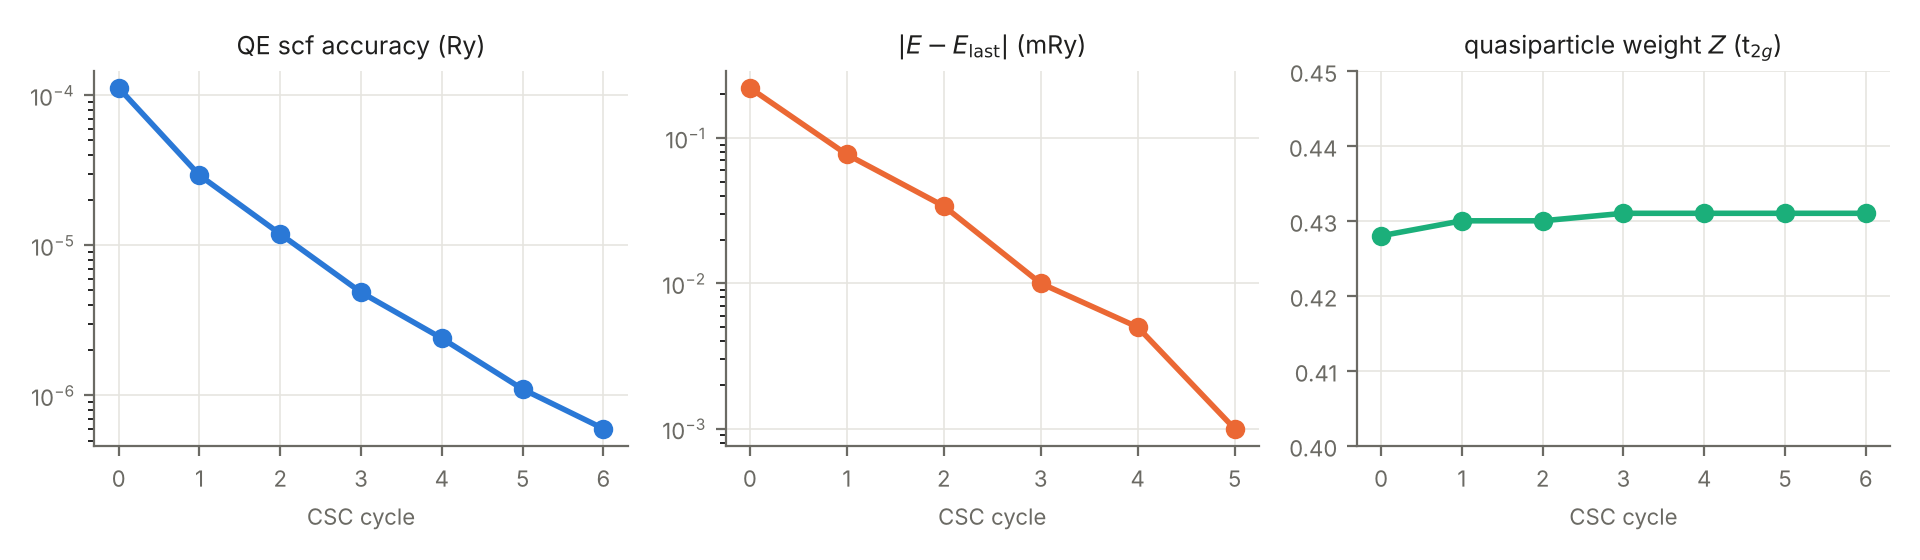
\includegraphics[width=\textwidth]{figures/qe_csc_srvo3.png}
\vspace{0.1cm}
\begin{itemize}\small
 \item geometric convergence: scf accuracy $6\times10^{-7}$ Ry after 7 cycles; window charge $=1$ throughout
 \item $Z$: 0.428 (one-shot) $\to$ 0.431 (CSC); $E_F$ shifts by $+12$ meV; small CSC effect, as for CaVO$_3$ (Beck 2022)
 \item limits: nspin $=1$ (QE hook); DMFT total energy not yet assembled
\end{itemize}
\end{frame}

\section{v1.3: closing the v1.2 list}
\begin{frame}{$\lambda$-corrected ladder D$\Gamma$A \refcite{Katanin, Toschi, Held, PRB 80, 075104 (2009)}}
\footnotesize
\[\chi_m^{\lambda}(\mathbf q,\omega)=\big[\chi_m(\mathbf q,\omega)^{-1}+\lambda_m\big]^{-1},\qquad
\tfrac1\bet\textstyle\sum_{\mathbf q\omega}\chi_m^\lambda(\mathbf q,\omega)=\tfrac1\bet\sum_\omega\chi_m^{\rm loc}(\omega)\]
\[\Sig(\mathbf k,\nu)=\Sig_{\rm DMFT}+\tfrac{\U}{\bet}\textstyle\sum_{\mathbf q\omega}\G(\mathbf k{+}\mathbf q,\nu{+}\omega)
\Big\{\tfrac12\big[1-\gamma_d(1-\U\chi_d)\big]-\tfrac32\big[1-\gamma_m(1+\U\chi_m^\lambda)\big]\Big\}+\dots\]
\centering
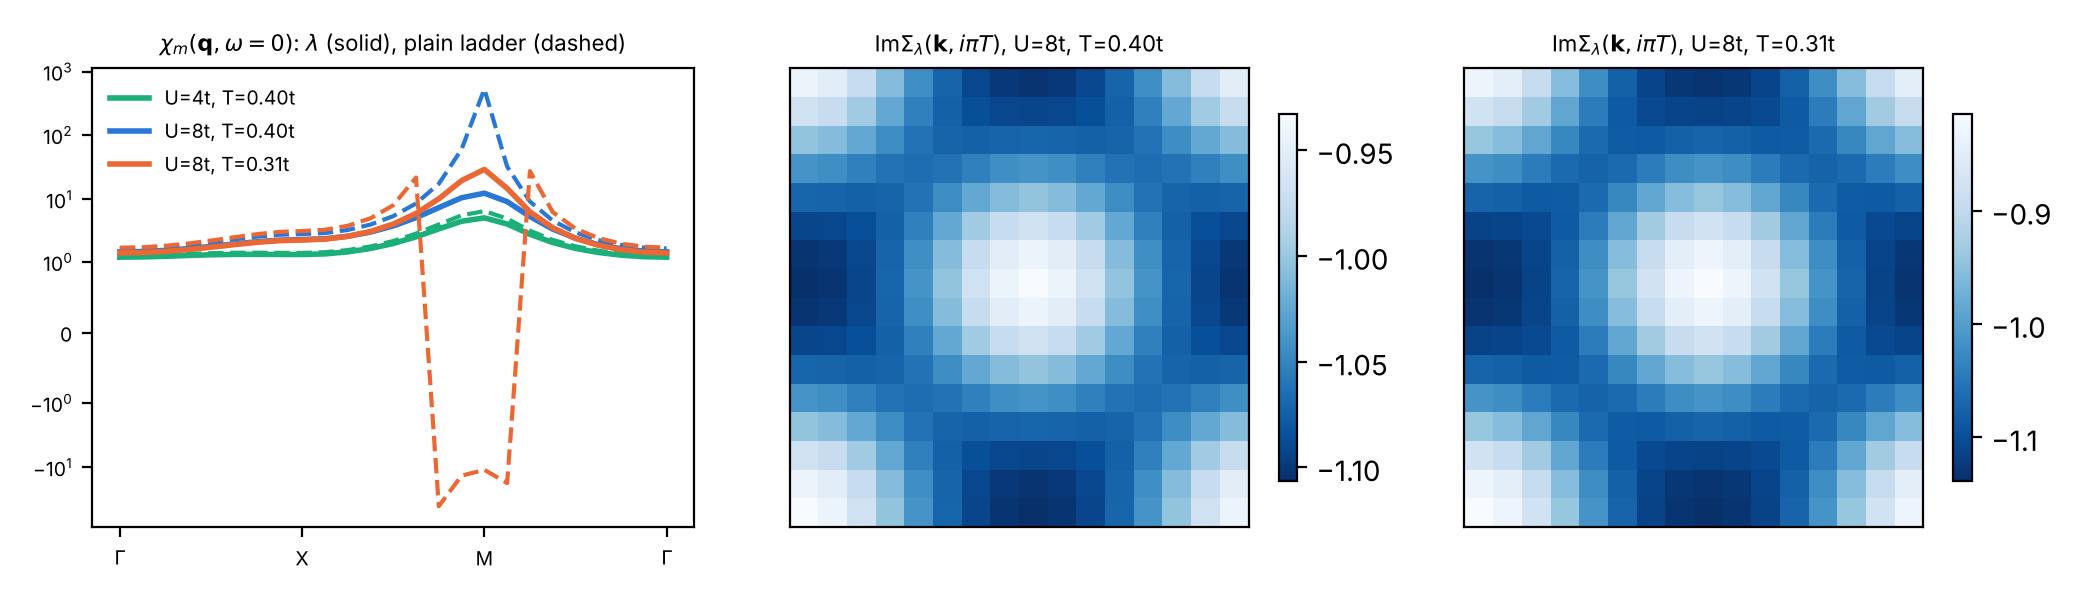
\includegraphics[width=0.98\textwidth]{figures/lambda_dga.png}
\begin{itemize}\scriptsize
 \item $\lambda=0$ reproduces the plain ladder to $4\times10^{-15}$; local spin sum rule restored exactly
 \item $\U=8t$, $T=0.31t$ (below $T_N^{\rm DMFT}$): plain ladder $\chi_m(Q)=-11$, Im$\Sig>0$; $\lambda$-D$\Gamma$A $\chi_m(Q)=29$ (Mermin--Wagner)
 \item $\U=4t$: $\chi_m(Q)$ within 25\% of TPSC; strongest scattering at the antinode
\end{itemize}
\end{frame}

\begin{frame}{5-orbital Kanamori CT-HYB \refcite{Haule 2007; S\'emon et al. 2014}}
\begin{columns}[T]
\column{0.5\textwidth}
\footnotesize
\[\mathrm{Tr}\big[e^{-(\bet-\tau_1)\Ham_{\rm loc}}O_1\cdots O_K e^{-\tau_K\Ham_{\rm loc}}\big]=\sum_{s_0}\mathrm{tr}_{s_0}[\dots]\]
\begin{itemize}\footnotesize
 \item $(N_\uparrow,N_\downarrow)$ blocks: each $c_f$, $c_f^\dagger$ maps one block to one block ($\le100$ states)
 \item bound $|\mathrm{tr}_{s_0}|\le d_{s_0}\prod\|B\|e^{-\Delta\tau E_{\min}}$: skip blocks, propagate only outer states with $e^{-\ell E_n}$ above tolerance
 \item lazy Metropolis: reject with the bound alone
 \item optional Haule truncation $E-E_0\le e_{\rm cut}$
\end{itemize}
\column{0.48\textwidth}
\footnotesize
\begin{tabular}{lll}
\toprule
5 orbitals, $\U=4$, $\J=0.6$ & ED ($2^{20}$) & CT-HYB\\\midrule
$\langle S_z^2\rangle$ & 1.933 & $1.936\pm0.008$\\
$\langle n_\uparrow n_\downarrow\rangle$ & 0.2179 & $0.2169\pm0.0012$\\
$n$ & 0.6090 & 0.6085\\
$e_{\rm cut}=10$: $\langle n_\uparrow n_\downarrow\rangle$ & 0.2075 & $0.2075\pm0.009$\\
\bottomrule
\end{tabular}

\vspace{0.2cm}
trace $=$ dense to $10^{-10}$; 3 orbitals: 349 s $\to$ 23 s (15$\times$)\\
5 orbitals: $\approx1$ ms per step at $\langle k\rangle\approx2$\\
\textcolor{muted}{G estimator noisy at low order (worm sampling: next)}
\end{columns}
\end{frame}

\begin{frame}{Vertex for continuous baths: $G_2$ from CT-HYB \refcite{Hafermann et al. 2012}}
\footnotesize
\[G_{2,\sigma\sigma'}(\nu,\nu',\omega)=\tfrac1\bet\big\langle \hat M_\sigma(\nu{+}\omega,\nu)\hat M_{\sigma'}(\nu',\nu'{+}\omega)-\delta_{\sigma\sigma'}\hat M_\sigma(\nu{+}\omega,\nu'{+}\omega)\hat M_\sigma(\nu',\nu)\big\rangle\]
\[\hat M(a,b)=\textstyle\sum_{ij}M_{ji}e^{i\nu_a\tau^e_i}e^{-i\nu_b\tau^s_j}\]
\begin{columns}[T]
\column{0.36\textwidth}
\begin{itemize}\scriptsize
 \item discrete bath vs Lehmann ED: deviations at the $1\sigma$ level; 16 s vs 292 s
 \item 3 bath sites: ED out of memory; CT-HYB: any $\Delta(i\omega)$
 \item Schwinger--Dyson: $\Sig_{\rm EOM}$ = $\Sig_{\rm Dyson}$ within 1--2\%
\end{itemize}
\column{0.62\textwidth}
\tiny
\begin{tabular}{@{}llll@{}}
\toprule
$\U=4t$, $T=0.4t$ & ED, box 16 & CT-HYB 16 & CT-HYB 32\\\midrule
sum target (exact 0.354) & 0.298 & 0.295 & 0.326\\
$\chi_m(Q)$ plain DMFT & 6.4 & 8.0 & 8.6\\
$\chi_m^\lambda(Q)$ box/exact & 5.0 / 10.8 & 5.1 / 11.3 & 5.7 / 8.0\\
Im$\Sig(\pi,0)$ box / exact & $-0.15/-0.27$ & $-0.13/-0.27$ & $-0.14/-0.20$\\
\bottomrule
\end{tabular}

\vspace{0.1cm}
larger box $\Rightarrow$ the two $\lambda$ targets converge (spread $2.2\to1.4$)
\end{columns}
\end{frame}

\section{Benchmarks, limitations, learning}
\begin{frame}{Benchmark philosophy}
\begin{columns}[T]
\column{0.5\textwidth}
\begin{itemize}\small
 \item every row: value, reference, error, tolerance, \textbf{citation}
 \item exact limits (atoms, $U=0$, sum rules) \emph{and} published results (PRL/PRB/RMP/EPL)
 \item cross-solver checks: CT-INT $\leftrightarrow$ CT-HYB $\leftrightarrow$ ED $\leftrightarrow$ NRG
 \item informational rows for approximations with known bias
\end{itemize}
\begin{block}{Three suites}
\small
\texttt{run\_benchmarks.py} --- 102 core checks (v0.1--v0.3)\\
\texttt{run\_v1\_benchmarks.py} --- 54 checks for the v1.0 modules (54/54 pass)\\
\texttt{run\_v11\_benchmarks.py} --- 43 checks closing the v1.0 limitations (43/43 pass)\\
\texttt{feynlab bench --suite all}
\end{block}
\column{0.47\textwidth}
\scriptsize
\begin{tabular}{ll}
\toprule
group & selected references\\\midrule
Diagrams & Molinari; Mattuck\\
Self-energy & Yamada--Yosida; Georges RMP 1996\\
QMC & Rubtsov 2005; Werner 2006\\
Mott & Bulla 1999; Karski 2005\\
NRG & Wilson 1975; Haldane 1978\\
Continuation & Fei--Yeh--Gull 2021\\
DiagMC & Rossi 2017/2018; Kozik 2015\\
Polaron & Mishchenko 2000\\
AHE & Sinitsyn 2007; Ado 2015\\
SHC & Sinova 2004; Inoue 2004\\
Orbitronics & Xiao 2007; Sodemann--Fu 2015\\
\bottomrule
\end{tabular}
\end{columns}
\end{frame}

\begin{frame}{Selected v1.0 benchmark rows}
\scriptsize
\renewcommand{\arraystretch}{1.1}
\begin{tabular}{llrrl}
\toprule
group & check & feynlab & reference & source\\\midrule
CT-HYB & $U=4$ double occupancy & 0.07805 & 0.07815 & ED\\
Kanamori & t$_{2g}^3$ ground state & 6.6 & $3U-9J=6.6$ & Georges et al.\ 2013\\
DCA & $N_c=1$ $Z$ & 0.486644 & 0.486638 & DMFT\\
two-particle & $\chi_0(0,0)$ & 0.208784 & $\partial n/\partial\mu$ & sum rule\\
NRG & Haldane slope & $-0.993$ & $-1$ & Haldane PRL 1978\\
NRG & local-moment plateau & 0.6877 & $\ln2$ & Krishna-murthy 1980\\
Nevanlinna & off-axis $G(2i)$ error & $6\times10^{-17}$ & 0 & Fei et al.\ 2021\\
CDet & atom $a_3$ & 0.16276 & 0.16276 & exact\\
resum & conformal map $x=3$ & 0.5 & 0.5 & Rossi 2018\\
polaron & $Z(\alpha=0.2)$ & 0.900 & $1-\alpha/2$ & perturbation theory\\
T-matrix & vs Born+skew & $-1.7265$ & $-1.7263$ & Sinitsyn 2007\\
crossed & lattice $X$ vs $k\!\cdot\!p$ & 0.795 & 0.790 & Ado 2015\\
OAM & Dirac valley moment & exact & & Xiao 2007\\
Edelstein & Rashba $|\delta S_y|$ & 0.023873 & $m\alpha/4\pi$ & Edelstein 1990\\
Wannier3D & stacked Chern & 0.333333 & $1/3$ & Halperin 1987\\
\bottomrule
\end{tabular}
\vspace{0.1cm}

{\scriptsize Full tables: \texttt{benchmarks/RESULTS.md} and \texttt{benchmarks/RESULTS\_v1.md}}
\end{frame}

\begin{frame}{Known limitations after v1.2 (stated honestly)}
\begin{columns}[T]
\column{0.5\textwidth}
\begin{itemize}\small
 \item QE CSC: nspin $=1$ only (QE hook); DMFT total energy not yet assembled
 \item CT-HYB vertex: single orbital, removal estimator (no worm sampling)
 \item $\lambda$-D$\Gamma$A: $\lambda_m$ only, box-size dependent
\end{itemize}
\column{0.47\textwidth}
\begin{itemize}\small
 \item sector CT-HYB: no tree caching; G estimator noisy at low order
 \item cluster CT-INT: usual sign problem off half filling, $N_c\ge4$
 \item finite-range disorder: semiclassical route only (Kubo--St\v{r}eda remains $\delta$-correlated)
\end{itemize}
\end{columns}
\vfill
\begin{block}{Next}
\small $\lambda_{dm}$-D$\Gamma$A, dual fermions, worm-sampled vertices and G, tree-cached traces, Kubo--St\v{r}eda with finite-range disorder
\end{block}
\end{frame}

\begin{frame}{Learning material}
\begin{columns}[T]
\column{0.5\textwidth}
\textbf{Software tutorials} (\texttt{docs/software\_tutorials})
\begin{enumerate}\scriptsize
 \item Getting started \quad 2.\ Diagrams \quad 3.\ Self-energy
 \setcounter{enumi}{3}
 \item CT-INT \quad 5.\ Hall transport \quad 6.\ Electron gas/BCS
 \setcounter{enumi}{6}
 \item Benchmarks \& limitations \quad 8.\ ED-DMFT Mott
 \setcounter{enumi}{8}
 \item Infrastructure \quad 10.\ CT-HYB, Kanamori, DFT+DMFT
 \setcounter{enumi}{10}
 \item DCA, two-particle, NRG \quad 12.\ Continuation
 \setcounter{enumi}{12}
 \item CDet, resummation, polaron \quad 14.\ Advanced transport
 \setcounter{enumi}{14}
 \item Matrix CT-HYB, cluster CT-INT, CSC, vertices \quad 16.\ v1.1 transport/continuation/polarons\\ \quad 17.\ QE charge self-consistency
\end{enumerate}
\textbf{Book tutorials}: every chapter 0--19 + appendices of Mattuck, with runnable feynlab companions.
\column{0.47\textwidth}
\begin{block}{Quizzes}
\small 42 quizzes, 228 questions with explanations: \texttt{quizzes/quiz.html} (self-contained, offline), \texttt{QUIZZES.md}, \texttt{quizzes.json}.
\end{block}
\begin{block}{Slides}
\small this deck: \texttt{docs/slides/feynlab\_slides.pdf} (source \texttt{.tex}, figures regenerated by \texttt{make\_figures.py})
\end{block}
\end{columns}
\end{frame}

\begin{frame}[fragile]{Getting started in five lines}
\begin{columns}[T]
\column{0.55\textwidth}
\scriptsize
\begin{verbatim}
git clone https://github.com/Gokaran-Shukla/feynlab
cd feynlab && pip install -e .
pytest -q                          # unit tests
feynlab hall --model dirac         # AHE mechanisms
feynlab bench --suite all          # every benchmark

from feynlab.dmft.bethe import BetheDMFT
r = BetheDMFT(beta=200, U=2.6).solve(
        'ed', ctint_kwargs=dict(n_bath=7))
print(r['Z'])
\end{verbatim}
\column{0.42\textwidth}
\begin{block}{Cite}
\small G.\ Shukla, \emph{feynlab: Feynman diagrams, QMC and Hall transport}, v1.2 (2026), github.com/Gokaran-Shukla/feynlab (see CITATION.cff)
\end{block}
\begin{block}{Roadmap}
\small $\lambda_{dm}$-D$\Gamma$A, dual fermions, worm-sampled vertices, finite-range Kubo--St\v{r}eda, cluster sign mitigation
\end{block}
\end{columns}
\end{frame}

\begin{frame}[plain]
\begin{tikzpicture}[remember picture,overlay]
 \fill[brand] (current page.south west) rectangle (current page.north east);
 \node[text=white,font=\Huge\bfseries] at (current page.center) {Thank you};
 \node[text=white!70!brand,font=\small] at ($(current page.center)+(0,-0.9)$) {github.com/Gokaran-Shukla/feynlab};
\end{tikzpicture}
\end{frame}

\end{document}
